\def\year{2016}\relax
%File: formatting-instruction.tex
\documentclass[letterpaper]{article}
\usepackage{aaai16}
\usepackage{times}
\usepackage{helvet}
\usepackage{courier}
\frenchspacing
\setlength{\pdfpagewidth}{8.5in}
\setlength{\pdfpageheight}{11in}
\pdfinfo{
/Title (Compressed Conditional Mean Embeddings for Model-Based Reinforcement Learning)
/Author (Guy Lever, John Shawe-Taylor, Ronnie Stafford, Csaba Szepesv\'{a}ri)} %
\setcounter{secnumdepth}{2}  




%%everything below and before \begin{document} is added by the authors

%% we are allowed to "minimally" make these spacing changes

\setlength\abovecaptionskip{0.2mm}
\setlength\belowcaptionskip{0mm}
\setlength\abovedisplayskip{0.2mm}
\setlength\belowdisplayskip{0.2mm}
\setlength\floatsep{0mm}
\setlength\textfloatsep{0.3mm}

%% Csaba's commands
%\usepackage[backgroundcolor = White]{todonotes}
\usepackage[disable]{todonotes}  %turn notes on/off with \usepackage[disable]{todonotes} 
% todo by Csaba
\newcommand{\todoc}[2][]{\todo[color=red!20!white,size=\tiny,#1]{#2}}
% todo by Guy
\newcommand{\todog}[2][]{\todo[inline,color=orange!20!white,size=\tiny#1]{#2}}
%\setlength{\marginparwidth}{10ex}
\usepackage{paralist}

%% Guys' commands
\usepackage{times}
\usepackage{graphicx}
%\usepackage{subfigure}
%\usepackage{caption}
\usepackage{subcaption} 
%\usepackage{natbib}
\usepackage{algorithm}
\usepackage{algorithmic}
%\usepackage{hyperref}
\usepackage{url}
\usepackage{bm}
\usepackage{latexsym}
\usepackage{amsmath,amsfonts,amssymb,color}
\usepackage{mathrsfs}
\usepackage{pifont}
\usepackage{amsthm}

\newtheorem{theorem}{Theorem}[section]
\newtheorem{lemma}[theorem]{Lemma}
\newtheorem{proposition}[theorem]{Proposition}
\newtheorem{corollary}[theorem]{Corollary}

%\newenvironment{proof}[1][Proof]{\begin{trivlist}
%\item[\hskip \labelsep {\bfseries #1}]}{\end{trivlist}}
\newenvironment{definition}[1][Definition]{\begin{trivlist}
\item[\hskip \labelsep {\bfseries #1}]}{\end{trivlist}}
\newenvironment{example}[1][Example]{\begin{trivlist}
\item[\hskip \labelsep {\bfseries #1}]}{\end{trivlist}}
\newenvironment{remark}[1][Remark]{\begin{trivlist}
\item[\hskip \labelsep {\bfseries #1}]}{\end{trivlist}}

%\newcommand{\qed}{\nobreak \ifvmode \relax \else
%      \ifdim\lastskip<1.5em \hskip-\lastskip
%      \hskip1.5em plus0em minus0.5em \fi \nobreak
%      \vrule height0.75em width0.5em depth0.25em\fi}

\newcommand{\vanHoofNonParametricControl}{DBLP:conf/aistats/Hoof0N15}
\newcommand{\CsabaFLAM}{DBLP:conf/adprl/YaoSPZ14}
\newcommand{\GrunewalderEmbeddingsRL}{GrunewalderEmbeddingsMDP}
\newcommand{\BertsekasApproximate}{BertsekasApproximate}
\newcommand{\BertsekasDynamic}{BertsekasDynamic}
\newcommand{\GrunewalderEmbeddingsRegression}{GrunewalderEmbeddingsRegression}
\newcommand{\SongNonparametric}{DBLP:journals/jmlr/SongGG10}
\newcommand{\SongKernelEmbedding}{DBLP:journals/spm/SongFG13}
\newcommand{\MichelliVectorValued}{DBLP:journals/neco/MicchelliP05}
\newcommand{\ParrLinear}{DBLP:conf/icml/ParrLTPL08}
\newcommand{\SuttonDyna}{sutton2008a}
\newcommand{\KroemerNonParametric}{DBLP:conf/nips/KroemerP11}
\newcommand{\DeisenrothPilco}{DBLP:conf/icml/DeisenrothR11}
\newcommand{\MallatMatchingPursuit}{DBLP:journals/tsp/MallatZ93}
\newcommand{\BengioKernelMP}{DBLP:journals/ml/VincentB02}
\newcommand{\ShaweTaylorBook}{DBLP:books/daglib/0026002}
\newcommand{\OrmoneitKBRL}{DBLP:journals/ml/OrmoneitS02}
\newcommand{\BarretoStochasticFactorization}{DBLP:conf/nips/BarretoPP11}
\newcommand{\KvetonRepresentativeKBRL}{DBLP:conf/aaai/KvetonT12}
\newcommand{\WatsonNadarayaWatson}{Wats:1964}
\newcommand{\NadarayaNadarayaWatson}{Nada:1964}
\newcommand{\ZhangMPConsistencey}{DBLP:journals/jmlr/Zhang09}
\newcommand{\HussainTheoryOfMP}{DBLP:conf/nips/HussainS08}
\newcommand{\BachLowRank}{DBLP:conf/icml/BachJ05}
\newcommand{\CsabaPersonalCommunication}{CsabaPersonalCommunication}
\newcommand{\BoydADMM}{DBLP:journals/ftml/BoydPCPE11}
\newcommand{\DuchiProjections}{DBLP:conf/icml/DuchiSSC08}
\newcommand{\BradtkeLSTD}{DBLP:journals/ml/BradtkeB96}
\newcommand{\BairdBRmin}{DBLP:conf/icml/Baird95}
\newcommand{\BellmanValueIt}{Bellman:1957}
\newcommand{\HowardPolicyIt}{howard:dp}
\newcommand{\LeverPoliciesInRKHS}{DBLP:conf/aistats/LeverS15}
\newcommand{\TibshiraniLasso}{tibshirani96regression}
\newcommand{\SinghEligibility}{DBLP:journals/ml/SinghS96}

\newcommand{\cD}{{\mathcal D}}
\newcommand{\cC}{{\mathcal C}}
\newcommand{\cB}{{\mathcal B}}
\newcommand{\cH}{{\mathcal H}}
\newcommand{\cF}{{\mathcal F}}
\newcommand{\cA}{{\mathcal A}}
\newcommand{\cS}{{\mathcal S}}
\newcommand{\cP}{{\mathcal P}}
\newcommand{\cV}{{\mathcal V}}
\newcommand{\cX}{{\mathcal X}}
\newcommand{\cM}{{\mathcal M}}
\newcommand{\cL}{{\mathcal L}}
\newcommand{\cE}{{\mathcal E}}
\newcommand{\cR}{{\mathcal R}}
\newcommand{\cG}{{\mathcal G}}
\newcommand{\br}{{\bm r}}
\newcommand{\bLambda}{{\bm \Lambda}}
\newcommand{\balpha}{{\bm \alpha}}
\newcommand{\bbeta}{{\bm \beta}}
\newcommand{\bZero}{{\bm 0}}
\newcommand{\bL}{{\bm L}}
\newcommand{\bV}{{\bm V}}
\newcommand{\bK}{{\bm K}}
\newcommand{\bM}{{\bm M}}
\newcommand{\bW}{{\bm W}}
\newcommand{\bR}{{\bm R}}
\newcommand{\bA}{{\bm A}}
\newcommand{\bI}{{\bm I}}
\newcommand{\bY}{{\bm Y}}
\newcommand{\bx}{{\bm x}}
\newcommand{\bF}{{\bm F}}
\newcommand{\bbb}{{\bm b}}
%\newcommand{\bB}{{\bm B}}
\newcommand{\bq}{{\bm q}}
\newcommand{\bPsi}{{\bm \Psi}}
\newcommand{\bPhi}{{\bm \Phi}}
\newcommand{\bw}{{\bm w}}
\newcommand{\E}{{\mathbb E}}
\newcommand{\R}{{\mathbb R}}
\newcommand{\Lin}{{\rm Lin}}
\newcommand{\loss}{\operatornamewithlimits{loss}}
\newcommand{\argmin}{\operatornamewithlimits{argmin}}
\newcommand{\argmax}{\operatornamewithlimits{argmax}}
\newcommand{\proj}{\operatornamewithlimits{proj}}
\newcommand{\greedy}{\operatornamewithlimits{greedy}}
\newcommand{\trace}{\operatornamewithlimits{tr}}
\newcommand{\lang}{\langle}
\newcommand{\rang}{\rangle}
\newcommand{\nn}{\nonumber}
\newcommand{\reg}{\operatornamewithlimits{reg}}
\newcommand{\bzero}{{\bm 0}}
\newcommand{\bone}{{\bm 1}}

%because I cannot use natbib
\newcommand{\citep}{\cite}
\newcommand{\citet}[1]{\citeauthor{#1} (\citeyear{#1})}

\begin{document}
% The file aaai.sty is the style file for AAAI Press 
% proceedings, working notes, and technical reports.
%
\title{Compressed Conditional Mean Embeddings for Model-Based Reinforcement Learning}
\author{Guy Lever \\ University College London \\ London, UK \\ g.lever@cs.ucl.ac.uk \And John Shawe-Taylor \\ University College London \\ London, UK \\ j.shawe-taylor@cs.ucl.ac.uk \And Ronnie Stafford \\ University College London \\ London, UK \\ r.stafford.12@ucl.ac.uk \And Csaba Szepesv\'{a}ri \\ University of Alberta \\ Edmonton, Canada \\ szepesva@cs.ualberta.ca  }
\maketitle

\begin{abstract} We present a model-based approach to solving Markov decision processes (MDPs) in which the system dynamics are learned using conditional mean embeddings (CMEs). This class of methods comes with strong performance guarantees, and enables planning to be performed in an induced finite (pseudo-)MDP, which approximates the MDP, but can be solved exactly using dynamic programming. Two drawbacks of existing methods exist: firstly, the size of the induced finite (pseudo-)MDP scales quadratically with the amount of data used to learn the model, costing much memory and time when planning with the learned model; secondly, learning the CME itself using powerful kernel least-squares is costly -- a second computational bottleneck. We present an algorithm which maintains a rich kernelized CME model class, but solves both problems: firstly we demonstrate that the loss function for the CME model suggests a principled approach to \emph{compressing} the induced (pseudo-)MDP, leading to faster planning, while maintaining guarantees; secondly we propose to learn the CME model itself using fast sparse-greedy kernel regression well-suited to the RL context. We demonstrate superior performance to existing methods in this class of model-based approaches on a range of MDPs.
\end{abstract}

\section{Introduction}

Several methods have been proposed for model-based reinforcement learning (RL) which, due to the form of the model, induce a finite (pseudo-)MDP\footnote{Pseudo-MDPs relax the potential transition functions from the set of probability measures to signed measures. See Section~\ref{InducedMDP}.} which approximates the MDP, such that solving the induced (pseudo-)MDP delivers a good policy for the true MDP \citep{\OrmoneitKBRL,\GrunewalderEmbeddingsRL,\CsabaFLAM}. In these methods the learned `model' can be viewed as a ``conditional mean embedding'' (CME) of the MDP transition dynamics. We review this family of methods in Section~\ref{CMEsforRL}.

In general the approach has the following potentially useful properties: 
\begin{inparaenum}[\itshape a\upshape)]
\item The induced finite approximate Bellman optimality equation can be solved exactly in finite time,
avoiding instability associated with approximate dynamic programming (e.g. \citet{\BertsekasApproximate}). As a result, planning is guaranteed to succeed.
\item Guarantees on the value of the learned policy exist: e.g. consistency in the large data limit for the algorithm of \citet{\OrmoneitKBRL} under mild smoothness assumptions or bounds on the value of the policy learned in terms of the error of the CME \citep{\GrunewalderEmbeddingsRL,\CsabaFLAM}. 
\item By reducing model learning to a supervised learning problem, to some extent the problem of a-priori defining a good compact representation architecture for value functions is avoided. %Here, value functions can be represented in rich reproducing kernel Hilbert space (RKHS) without explicitly constructing feature vectors.
\todoc{But the algorithm DOES compute a value function! Take this out?}\todog{Yes OK its a bit confusing. I mention this later so have just removed it here. OK?} \todoc{Yep, I removed the last sentence.}
\item The approach can be data-efficient since state-of-the-art non-parametric approaches can be used to approximate the CME from few data points.
\end{inparaenum}

One drawback is the fact that the size of the induced finite (pseudo-)MDP scales quadratically with the amount of data used to learn the model, significantly slowing down the planning step and straining the algorithm's memory requirements as more data is collected. Further, \citet{\GrunewalderEmbeddingsRL} employ non-parametric methods to learn the CME which are data efficient but computationally expensive. \todoc{Did not this paper also talk about using sparsification techniques?}\todog{Yes, I'll try to fit a discussion of this in but because of space we may have to only mention this if reviewers bring it up.}
\todoc{What will you say? Maybe we can fit it somewhere..}
 It is therefore of interest to investigate methods for learning CMEs in RL which retain these benefits but enable efficient planning and which can be learned efficiently even for problems that require huge amounts of data to learn a good model. We present a method of learning a \emph{compressed CME} which induces a compressed finite pseudo-MDP for efficient planning, decoupling the amount of data collected and the size of the induced pseudo-MDP. The compression guarantees the existence of compressed CMEs maintaining good performance bounds. We optimize the CME non-parametrically but efficiently, using kernel matching pursuit.

\section{Preliminaries}

\subsection{Reinforcement Learning Background} \label{RLbackground}

We recall basic concepts associated with reinforcement learning (RL). In RL an agent acts in an environment by sequentially choosing actions over a sequence of time steps, in order to maximize a cumulative reward. We model this as a \emph{Markov decision process} (MDP) which is defined using 
a \emph{state space} $\cS$, 
an \emph{action space} $\cA$, 
an \emph{initial state distribution} $P_1$ over $\cS$, 
an \emph{(immediate) reward function} $r:\cS \times \cA \to [0,1]$,
and a stationary \emph{Markov transition kernel} $(P(s' |s,a))_{(s,a,s')\in \cS \times \cA \times \cS}$
These, together with a (stationary, stochastic, Markov) policy $\pi: \cS \to \cP(\cA)$, a map from the state space to the set of distributions over the action space, gives rise to a controlled Markov chain $\xi=(S_1,A_1,S_2,A_2,\dots)$ where $S_1 \sim P_1$, $A_t \sim \pi(S_t)$ and $S_{t+1} \sim P(\cdot|S_t,A_t)$, i.e., $P$ determines the stochastic dynamics of the controlled process.
% $P(S_{t+1}|S_i=s_i, A_i=a_i ,\forall i\le t) = P(S_{t+1} |S_t=s_t,A_t=a_t)$; a (potentially stochastic) \emph{reward function} $R:\cS\times\cA\to \R$. We denote the mean of the reward function by $r(s,a) = \E [R(s,a)]$, and use the shorthand $P(S_{t+1} |s_t,a_t) = P(S_{t+1} |S_t=s_t,A_t=a_t) $ and 
%Given an MDP, an \emph{agent} controls a \emph{trajectory} $\xi = (s_1,a_1,s_2,a_2,...)$ through $\cS\times\cA$ by sequentially selecting the actions $a_t\in\cA$ at each time step according to a stationary \emph{policy} $\pi:\cS\to\cP(\cA)$, where $\cP(\cA)$ is the set of probability distributions on $\cA$. 
An \emph{agent} that interacts with an MDP observes (some function of) the states and selects actions sequentially with the goal 
to accumulate reward comparable to what could be obtained by a policy $\pi^*$ which maximizes the \emph{expected return} (expected total cumulative discounted reward), $J(\pi):= \E [\sum_{t=1}^\infty \gamma^{t-1} r(S_t,A_t) ; \pi]$ where,  $\E [ \cdot ; \pi]$ denotes the expectation with respect to $P_1$, $P$ and $\pi$. We recall the \emph{value function} $V^\pi(s) :=  \E [\sum_{t=1}^\infty \gamma^{t-1} r(S_t,A_t) | S_1 =s ; \pi]$ and \emph{action-value function} $Q^\pi(s,a) := r(s,a) + \gamma \E_{S'\sim P(\cdot|s,a)} [V^\pi(S')]$
(generally, we will denote the successor state of $s$ by $s'$).
The \emph{optimal value function} is defined by $V^*(s) = \sup_{\pi\in\Pi} V^\pi(s)$.
For a given action-value function $Q:\cS\times\cA\to\R$ we define the (deterministic) \emph{greedy policy} w.r.t. $Q$ by $\pi(s) := \argmax_{a\in\cA} Q(s,a)$ and denote $\pi = {\greedy}(Q)$ (ties broken arbitrarily). 
Obtaining $V^\pi$ for a given $\pi$ is known as \emph{value estimation}. Any $V^\pi$ satisfies the \emph{Bellman equation},
\begin{align}
V^\pi(s) = \E_{A\sim\pi(s)} [ r(s,A) + \gamma \E_{S'\sim P(\cdot|s,A)} [V^\pi(S')] ], \label{BellmanExpectation} 
\end{align}
and the map $T^{\pi}:\cV\to\cV$, over the set $\cV$ of real-valued functions on $\cS$, defined by $(T^{\pi}V)(s):=  \E_{A\sim\pi(s)} [ r(s,A) + \gamma \E_{S'\sim P(\cdot|s,A)} [V(S')] ] $ is known as the Bellman operator for $\pi$. 
For finite state spaces an \emph{optimal policy} can be obtained using dynamic programming methods such as value iteration \citep{\BellmanValueIt} and policy iteration \citep{\HowardPolicyIt}. In policy iteration $V^\pi$ is obtained by solving (\ref{BellmanExpectation}) for a given deterministic policy $\pi:\cS\to\cA$ followed by taking the greedy policy with respect to $V^\pi$ and iterating.
In MDPs with large or continuous state spaces, value functions are typically represented in some approximation architecture, e.g., as a linear function in some feature space, $V^\pi(s)\approx  \lang v_\pi,\phi(s) \rang_\cF =: \hat V^\pi(s)$ where $\phi:\cS\to\cF$ is a feature map, and $\cF$ a Hilbert space. Choosing a feature map $\phi(\cdot)$ a-priori can be a problem since it is difficult to balance powerful representation ability and parsimoniousness. \todoc{We still do this. So maybe reword/clarify. Maybe RKHSs ameliorate this issue, but RKHS spaces are still quite small, or if they are big, learning will be super-slow. My view is that RKHS removes an artificial requirement that the feature map should be finite dimensional and thus increases flexibility, but this is all.}\todog{Not Sure I understand. We don't pick a compact $\cF$. I guess you can do kernel LSTD which avoids the compactness, is that what you mean? I could say hard to balance representation, compactness/computational efficiency? We don't really have that trade-off to worry about.} \todoc{We do -- see email.}
Further, in the approximate case value estimation entails solving
\begin{align}
&\lang w_\pi , \phi(s) \rang_{\cF}\hspace{-0.5mm}\approx \hspace{-0.5mm}r(s,\pi(s)) \hspace{-0.5mm}+\hspace{-0.5mm}  \gamma \E_{S'\sim P(\cdot|s,\pi(s))} [\lang v_\pi , \phi(S')\rang_{\cF}] ,\nn
%&\quad=r(s,\pi(s)) +  \gamma \lang v_\pi , \E_{S'\sim P(\cdot|s,\pi(s))} [\phi(S')]\rang_{\cF}, 
\end{align}
which must be solved approximately (using, for example, LSTD \citep{\BradtkeLSTD} or minimizing the Bellman residual \citep{\BairdBRmin}) since in general no solution in $v_\pi$ can be found with equality for a given feature map $\phi(\cdot)$, which can lead to instabilities \citep{\BertsekasDynamic}.

\emph{Model-based} reinforcement learning is an approach to RL in which data is used to estimate the dynamics and/or reward function followed by solving the resulting estimated MDP. This approach can be data efficient since the planning stage can be performed offline, and does not require interaction with the system. In this work we will present a model-based policy iteration algorithm \todoc{Policy, value iteration, or even linear programming: It does not matter (much) what we choose. Maybe this should be clarified at some point; in the summary?}
with a particular form of the transition model. We suppose that the mean reward function $r$ is known. Trivially, any estimate for the mean reward function can be substituted into our algorithm. 

\subsubsection{Related Work}
The approaches most similar to ours are by \citet{\OrmoneitKBRL}, \citet{\GrunewalderEmbeddingsRL} and \citet{\CsabaFLAM} and we defer a detailed discussion to Section~\ref{learningCMEs}. Related dynamics models which estimate expected successor feature maps using regression are common in approximate dynamic programming \citep{\ParrLinear,\SuttonDyna}. The key difference is that we will use the model to solve an MDP by deriving an induced finite pseudo-MDP and solving it exactly. Further, we separate the dynamics learning from any particular policy. A similar idea was explored recently by 
 \citet{\vanHoofNonParametricControl} in the context of a direct policy search algorithm.

%In \cite{\KroemerNonParametric} modeling dynamics for value estimation is considered, and the joint distribution over $(s,a,s')$ is modeled using kernel density estimation. This density is composed with dynamic programming to learn a value function. Kernel density estimates can be powerful, but the kernel approach scales cubicly with the amount of data and involves potentially difficult integrals over the state space -- we aim for alternative methods which scale linearly in the amount of data. Further, we adopt an approach in which the transition dynamics are learned independently of a particular policy so can be reused during policy optimization.

%In \cite{\DeisenrothPilco} a Gaussian process (GP) is used to model the transition dynamics. The aim here is to minimize the interaction required with the system, and a good dynamics model is learned with relatively few interactions. The underlying GP model however again scales cubicly in the number of datapoints, which will limit scalability. We adopt a different approach in which we suppose data is more abundant and aim for a method capable of processing huge amounts of data, and incorporating online data efficiently.

\section{Conditional Mean Embeddings for RL} \label{CMEsforRL}

The representation of the model that we study in this work is motivated by dynamic programming algorithms. In policy iteration the model is required to solve the Bellman expectation equation (\ref{BellmanExpectation}), and so it is sufficient to compute the conditional expectation of value functions, $\E_{S'\sim P(\cdot|s,a)}[V(S')]$. %Under the assumption that value functions of interest reside in a Hilbert space $\cF$, a natural loss function for any estimator $\hat E:\cF\times (\cS\times\cA)\to \R$ of the conditional expectation operator $(f,(s,a)) \mapsto \E_{S'\sim P(\cdot|s,a)}[f(S')]$ is therefore
%\begin{align}
%\loss(\hat E):= \sup_{V\in\cF:||V||\le 1} \E_{(s,a)\sim D}[ ( \hat E(V,(s,a)) - \E_{S'\sim P(\cdot|s,a)}[V(S')] )^2 ], \nn
%\end{align}
%where $D$ is some data distribution.
Recalling the discussion in Section~\ref{RLbackground}, when $V(s)= \lang v,\phi(s) \rang_{\cF}$, we have that $\E_{S'\sim P(\cdot|s,a)}[V(S')] = \lang \E_{S'\sim P(\cdot|s,a)}[\phi(S')] , v \rang_\cF$ and hence it suffices to learn the function $\mu:\cS\times\cA\to\cF$ such that 
\begin{align}
\mu(s,a) = \E_{S'\sim P(\cdot|s,a)}[\phi(S')]. \label{muDef}
\end{align}
In this work our ``transition model'' is an estimate of $\mu(\cdot)$, and for any estimate $\hat \mu(\cdot)$ we write,
\begin{align}
\hat E_{\hat\mu}(V,(s,a)) =  \lang \hat \mu(s,a) , v \rang_\cF \approx  \E_{S'\sim P(\cdot|s,a)}[V(S')]\,, \label{hatEDef}
\end{align}
where we used the (so-far implicit) convention that $V(s) =\lang v, \phi(s) \rang_{\cF}$.
Note that $\hat E_{\hat\mu}$ may not correspond to any conditional probability measure on $\cS$. The loss
\begin{align}
\loss(\hat \mu) := \E_{(s,a)\sim D, s' \sim P(\cdot|s,a)}[ || \hat\mu (s,a) - \phi(s') ||_\cF^2 ], \nn
\end{align}
where $D$ is some data distribution over $\cS \times \cA$, serves as a natural objective for the problem of learning $\mu(\cdot)$ \citep{\GrunewalderEmbeddingsRegression}. Given data\footnote{We will use the (sloppy) notation $s'_i\in\cD$ to indicate the successor states in $\cD$ in the sense that $s'_i\in\cD \Leftrightarrow\exists (s_i,a_i,s'_i)\in\cD$, and similarly for the actions $a_i$, and predecessor states $s_i$.} $\cD = \{(s_i,a_i,s'_i)\}_{i=1}^n$, where $s'_i\sim P(\cdot|s_i,a_i)$ the empirical loss is therefore,
\begin{align}
\widehat\loss(\hat \mu) := \frac{1}{n}\sum_{i=1}^n || \hat\mu (s_i,a_i) - \phi(s'_i) ||_\cF^2. \label{EmpMuObjective}
\end{align}
The function $\mu(\cdot)$ defined in (\ref{muDef}) is known as the \emph{conditional mean embedding} (CME) of $P$ in $\cF$; methods to learn CMEs have been provided by \citet{\SongKernelEmbedding} and \citet{\GrunewalderEmbeddingsRegression}.

%Modeling the transition dynamics by learning the CME enjoys some potentially useful properties in the reinforcement learning framework, which we now discuss.

\subsection{Key Properties of the CME Approach}

\subsubsection{The Induced Finite (Pseudo-)MDP} \label{InducedMDP}

As we will see in Section~\ref{learningCMEs}, several approaches to learn the CME (\ref{muDef}) from data result in a solution of the form $\hat \mu(s,a) = \sum_{i=1}^n \alpha_i(s,a) \phi(s'_i)$. This means that, from (\ref{hatEDef}),
\begin{align}
\hat E_{\hat\mu}(V,(s,a)) = \lang \hat \mu(s,a) , v \rang_\cF =\sum_{i=1}^n \alpha_i(s,a) V(s'_i), \label{finiteExpansion}
\end{align}
i.e., our estimates of conditional expectation can be computed by measuring $V$ only on the sample points $\{ s_i'\}_{i=1}^n$. In fact $\alpha_i(s,a)$ can be viewed as the ``probability''\footnote{The $\alpha_i(s,a)$ are not necessarily positive or normalized.} of transitioning to state $s'_i$ from state-action $(s,a)$ under the learned model (and the probability of transitioning to states beyond the sample is zero). Collect $(\alpha_i(s,a))_{i=1}^n$ into the vector $\balpha(s,a)\in \R^n$.
If, further,
\begin{align}
||\balpha(s'_i,a)||_1 \le 1 \label{L1Constraint}
\end{align}
for all successor states $s'_i\in\cD$ and $a\in\cA$ then the approximation  $\hat T^\pi_{\hat \mu}\hspace{-0.6mm}:\hspace{-0.6mm}\cV\hspace{-0.9mm}\to\hspace{-0.9mm}\cV$ of the Bellman operator $T^\pi$ defined by
\begin{align}
(\hat T^\pi_{\hat \mu}V)(s)&:=  \E_{A\sim\pi(s)} [ r(s,A) + \gamma \hat E_{\hat \mu}(V, (s,A))] \nn\\
&= \E_{A\sim\pi(s)} [ r(s,A) + \gamma \sum_{i=1}^n \alpha_i(s,A)V(s_i') ] \label{approxBellman}
\end{align}
is a contraction on the sample and so iterated ``backups'' $V\leftarrow \hat T^\pi_{\hat \mu}V$ will converge to a fixed point $\hat V_{\hat \mu}^{\pi}$ such that $\hat V_{\hat \mu}^{\pi} = \hat T^\pi_{\hat \mu} \hat V_{\hat \mu}^{\pi}$. The solution to the fixed point equation
\begin{align}
V =  \hat T^\pi_{\hat \mu} V \label{approxFP}
\end{align}
can be determined exactly by solving a linear system in $n$ variables by matrix inversion (or approximately by iterating backups): i.e. to perform this version of policy iteration the value function only needs to be maintained at the successor sample points $s'_i\in\cD$, even if $\cS$ is continuous. This should be contrasted to the typical situation in approximate dynamic programming, in which the Bellman equation cannot be solved exactly in general, and backups followed by projection can diverge. For the same reason the greedy policy can be executed anywhere on $\cS$ using knowledge of $\hat V_{\hat \mu}^{\pi}(\cdot)$ only at the sample points $s'_i\in\cD$ since we can construct the corresponding action-value function at any state-action, via
\begin{align}
\hat Q_{\hat \mu}^{\pi}(s,a) = r(s,a) + \gamma \sum_{i=1}^n \alpha_i(s,a)\hat V_{\hat \mu}^{\pi}(s_i').\label{Qapprox}
\end{align}
We refer to a CME such that $\sum_j |\alpha_j(s,a)| \le 1$ for all $(s,a)\in\cS\times\cA$ a \emph{proper CME}. When $\alpha_j(s_i',a)\ge 0$ and  $\sum_k \alpha_k(s_i',a) = 1$ for all $i,j$, $\hat T^{\pi}_{\hat \mu}$ is the Bellman operator for an MDP defined on the sample $\{s'_i\}_{i=1}^n$, whose dynamics are defined by $P(s_j'|s_i',a) = \alpha_j(s_i',a)$. Otherwise $\alpha_j(s_i',a)$ does not define an MDP, hence we refer to the induced \emph{pseudo-MDP} in general. A theory of pseudo-MDPs, as a method of MDP abstractions, has been developed in \citet{\CsabaFLAM}. 
A few important results include the following: The condition that makes CMEs proper allows one to define value functions for policies the usual fashion (with expectation w.r.t. signed measures). The value functions satisfy the analog Bellman equations. If one defines the optimal value function as the fixed-point of the analogue Bellman optimality equation then this optimal value function can be found by value-iteration.
\todoc{Actually, maybe this paper does not cover all these, due to space limits.. Brr..}\todog{OK.}
One can also show that value-iteration can be replaced by either linear programming or policy iteration under, e.g., the additional condition that $\alpha_j$ is nonnegative valued.

\subsubsection{Policy Iteration using CMEs} \label{PolItSec}

These observations motivate a generic model-based policy iteration algorithm for solving MDPs using CMEs: Collect data to learn an approximate proper CME (\ref{muDef}) of the transition dynamics; solve the approximate Bellman equation (\ref{approxBellman}) on the samples exactly; Construct the approximation (\ref{Qapprox}) and take the greedy policy $\greedy(\hat Q_{\hat \mu}^{\pi})$; iterate if necessary. For clarity this is outlined in pseudocode in Algorithm~\ref{GenericPolIt}.

\begin{algorithm}[htb]
   \caption{Generic model-based policy iteration with CMEs}
   \label{GenericPolIt}
\begin{algorithmic}
   \STATE {\bf Input:} MDP $\cM = (\cS,\cA,P_1,P,R)$ to interact with; known mean reward function $r$, known start-state distribution $P_1$.
	 \STATE {\bf Initialize:} $Q_0=r$, $\cD_0 = \emptyset$, $\hat P^0$, $\pi_1 = \greedy(Q_0)$
   \STATE {\bf Parameters:} $n_{\rm new}$, $J$\\
	 \FOR {$k=1,2,...$}
	 \STATE {\bf Data acquisition:} Collect $n_{\rm new}$ data points $\cD_{\rm new}$ (e.g. from the policy $\pi_k$ or an exploratory policy). Aggregate data: $\cD_k = \cD_{k-1}\cup\cD_{\rm new}$.
	 \STATE {\bf Update dynamics model:} Learn the CME $\hat \mu(\cdot)$ using the data $\cD_k$.
	\FOR {$j=1,2,...,J$}
   \STATE {\bf Policy evaluation:} Form estimate $\hat V_j$ of $V^{\pi_k}$ by solving the approximate Bellman Equation $V =  \hat T^\pi_{\hat \mu} V$ (\ref{approxFP}). Define $\hat Q_j(s,a) = r(s,a) + \gamma \sum_{j=1}^n \alpha_j(s,a) \hat V_j(s_j')$.
	 \STATE {\bf Policy improvement:} $\pi_{k} \leftarrow \greedy(\hat Q_j)$. 
   \ENDFOR
	 \STATE $\pi_{k+1} \leftarrow \pi_{k} $.
	\ENDFOR
\end{algorithmic}
\end{algorithm}

\subsubsection{Modeling Value Functions}

Although we assume value functions can be well-approximated in $\cF$, we never need to model them in $\cF$, i.e. find a weight vector $v$ such that $\lang v,\phi(s)\rang_{\cF} \approx V(s)$. We will see that it is not even necessary to construct $\phi(s)$ for any $s$, knowledge of the kernel function $L(s,s') = \lang \phi(s),\phi(s') \rang$ is sufficient. Thus the approximation space $\cF$ for $V$ can be a rich function class.

\subsubsection{Performance Guarantees}\label{PerformanceGuarantees}

It is possible to derive bounds on the value of the learned policy in value iteration \todoc{Not the best that this is not about policy iteration}
 in terms of the quality of the learned model and how well $V^*$ can be modeled in $\cF$. For example we have the following theorem:
\begin{theorem}{(\citet{\GrunewalderEmbeddingsRL}, Theorem 3.2)} %; see also \citet{\CsabaFLAM})} 
\label{ICMLtheorem}
Let $\hat V_k$ be the $k$th function obtained 
after $k$ iterations of value iteration using a proper CME $\hat\mu$, $\epsilon = \sup_{s,a} ||\mu(s,a) - \hat\mu(s,a)||_{\cF}$,
$\alpha = \|\hat V_1 - \hat V_0\|_\infty$,
 and let $\pi_k = \greedy(\hat V_k)$ be the resulting greedy policy. Then, for any  $\tilde V^*\in \cF$,
\begin{align*}
&||V^{\pi_k} \hspace{-0.6mm}-\hspace{-0.6mm} V^*||_{\infty}
\le \frac{2\gamma}{1-\gamma^2}\Big( \gamma^k
%	 ||\hat V_1 \hspace{-0.6mm}-\hspace{-0.6mm} \hat V_0||_{\infty} 
	 \alpha
	 \hspace{-0.6mm}+ \hspace{-0.6mm}2|| V^* \hspace{-0.6mm}-\hspace{-0.6mm} \tilde V^* ||_{\infty} 
	 +\epsilon ||\tilde V^*||_{\cF} \Big)\,. %\label{ICMLbound}
\end{align*}
\end{theorem}
Theorem~\ref{ICMLtheorem} applies to any proper estimate of the CME, independently of how it is learned.\todoc{But does not this hold when $\sup_{s,a} ||\mu(s,a) - \hat\mu(s,a)||_{\cF}$ is small for similar methods? In some sense, the requirement that this is small is the same that for any policy, the value function can be well approximated. This actually follows from the previous result, does not it?}\todog{Complicated. I've sent an email, but removed this for now.}

\subsection{Review of Current Approaches} \label{learningCMEs}

We now review the current approaches to learning the CME in model-based reinforcement learning algorithms which result in solving finite MDPs.

\subsubsection{Kernel-Based Reinforcement Learning}

The idea of using an induced finite MDP from a model estimate was, to our knowledge, introduced in the Kernel-Based Reinforcement Learning algorithm (KBRL) of \citet{\OrmoneitKBRL} 
\todoc{The same idea was used by John Rust, though in the context of planning, not for estimating a model.
See \citet{rust96:randomization} and \citet{sze01:planning}. Also, state space discretization is the same idea.
}\todog{I added this as a footnote, but we are short of space so may have to drop it, until after reviews. Is it vital for now?}
who derive an approximate finite Bellman equation induced by a model and solve it.\footnote{The same idea was used by \citet{rust96:randomization} and \citet{sze01:planning}, though in the context of planning, not for estimating a model.}
The model can be viewed as approximating the CME (\ref{muDef}) using kernel smoothing (i.e. a Nadaraya-Watson regressor),
\begin{align}
\hat\mu^{KBRL} (s,a)\hspace{-0.3mm}:= \hspace{-0.3mm}\sum_{i=1}^n\hspace{-0.3mm} \frac{K((s,a),(s_i,a_i))}{\sum_{j=1}^n K((s,a),(s_j,a_j))}\phi(s'_i), \label{KBRLmu}
\end{align}
where $K$ is a smoothing kernel.  \todoc{I did not double check whether this is indeed the same as what they do. But I guess it is the same..} 
No loss function is directly specified or optimized. The induced finite transition dynamics are given by $\alpha^{KBRL}_i(s,a) :=  \frac{K((s,a),(s_i,a_i))}{\sum_{j=1}^n K((s,a),(s_j,a_j))}$ and condition (\ref{L1Constraint}) holds. The KBRL method is shown to be consistent: the learned value function will converge to the optimal value function with infinite data.

One drawback of the approach is that the size of the state space of the induced MDP equals $|\cD|=n$ and planning via a solving the approximate Bellman equation (\ref{approxBellman}) scales poorly with the data. Versions of KBRL with efficient planning have been proposed using stochastic factorization of the transition matrix of the induced finite MDP \citep{\BarretoStochasticFactorization} or a cover tree quantization of the state space \citep{\KvetonRepresentativeKBRL}.

\subsubsection{Modeling Transition Dynamics with Kernel Least Squares CMEs}

\citet{\GrunewalderEmbeddingsRL} suggest a regularized least squares approach to learning the CME (\ref{muDef}) applying methods from the literature on learning CMEs \citep{\SongKernelEmbedding,\GrunewalderEmbeddingsRegression}. In general, a normed hypothesis class $\cH\subset \cF^{\cS\times\cA}$ is chosen and the empirical loss (\ref{EmpMuObjective}) plus a regularization term is minimized,
\begin{align}
\hat\mu^{RLS}\hspace{-0.9mm} := \hspace{-0.6mm}\argmin_{\mu\in\cH}  \hspace{-0.7mm}\frac{1}{n}\hspace{-0.7mm}\sum_{i=1}^n\hspace{-0.6mm} || \mu (s_i,a_i) \hspace{-0.7mm}-\hspace{-0.7mm} \phi(s'_i) ||_\cF^2 \hspace{-0.7mm}+\hspace{-0.7mm}\lambda ||\mu||^2_{\cH} . \label{muRLS}
\end{align}
When $\cH=\cH_K$ is a RKHS (of $\cF$-valued functions) with a kernel $K$ on $\cS\times\cA$ the solution to (\ref{muRLS}) is $\hat\mu^{KRLS}(s,a) = \sum_{j=1}^n \alpha_j^{KRLS}(s,a) \phi(s'_j)$ where
\begin{align}
\alpha_j^{KRLS}(s,a) &=  \sum_{i=1}^n K((s,a),(s_i,a_i)) W_{ij}  \label{KRLSalphas}
\end{align}
where $\bW = (\bK + \lambda \bI)^{-1}$, and $K_{ij} = K((s_i,a_i),(s_j,a_j))$ is the kernel matrix on the data. The approach to guarantee the constraint (\ref{L1Constraint}) is simply to threshold and normalize the $\alpha(s_i',a)$ for all $s_i'\in\cD$ and $a\in\cA$, in practice, however, we find it is better to project the weights using fast Euclidean projection to the L1-ball \citep{\DuchiProjections}, followed by normalization. %However, if computationally feasible, we find it is much better in practice to project the learned next feature map $\hat\mu^{KRLS}(s,a) \approx \E[\phi(S')|s,a]$ to obtain a proper CME:
%\begin{align}
%\balpha^{PKRLS}(s,a) &:= \argmin_{\bbeta \in \R^n} || \hat\mu^{KRLS}(s,a) - \sum_{j=1}^n \beta_j  \phi(s'_j)  ||_{\cF}, \nn\\
%&=\argmin_{\bbeta \in \R^n} || \sum_{j=1}^n \alpha_j^{KRLS}(s,a) \phi(s'_j) - \sum_{j=1}^n \beta_j  \phi(s'_j)  ||_{\cF}, \label{projectedAlpha} \\
%\hat\mu^{PKRLS}(s,a) &= \sum_{j=1}^n \alpha_j^{PKRLS}(s,a) \phi(s'_j). \nn
%\end{align}
%and solve the finite (pseudo-)MDP induced by the projected CME. We write $\balpha^{PKRLS}(s,a) = {\rm proj}(\balpha^{KRLS}(s,a))$. This essentially finds the closest feature in $\cF$ to that predicted by the regularized kernel least squares model but which is proper and so guarantees a contraction. Problem (\ref{projectedAlpha}) can be solved using a Lasso \citep{\TibshiraniLasso}, see Appendix~\ref{LassoSec}.
Unlike KBRL \citep{\OrmoneitKBRL} this approach minimizes a loss over a rich hypothesis class.

\iffalse
Indeed potentially very rich hypothesis classes such as deep neural networks could be used in much the same least-squares CME framework. The approach can be data-efficient since state-of-the-art techniques are used to learn the CME using few data points. However, in addition to the poor scaling of planning in the induced finite MDP, learning the model itself is of cubic computational complexity in the total amount of data. The online nature of data acquisition in RL presents a problem since a full relearn of the CME cannot practically be performed every policy/value iteration. However more efficient online updates to the model can be performed\footnote{In the same manner as online updates to kernel least square regressors.}, in which case each update is of quadratic complexity; model selection then becomes problematic since the CMEs for all possible parameters (i.e. a grid of kernel bandwidths and regularization parameters) must be stored and updated at each iteration, leading to large memory requirements. In \citet{\GrunewalderEmbeddingsRL} the approach is considered in the batch setting, in which good system data is provided a-priori the learning process.

One special case which is interesting for purposes of comparison with other work is when the kernel is induced by a finite dimensional feature map, and the CME is learned in the primal:
\begin{theorem}\label{Ftheorem} Suppose $K((s,a),(s',a')) = \psi(s,a)^\top \psi(s',a')$ for some feature map $\psi:\cS\times\cA\to\R^d$. In this case the solution to (\ref{muRLS}) is $\hat\mu^{RLS}(s,a) = \sum_{j=1}^n\alpha_j^{RLS}(s,a)\phi(s_j')$ where $\alpha_j^{\rm RLS}(s,a) = \psi(s,a)^\top \hat\bF_i$ and $\hat\bF = (\bF_1,...,\bF_n)$ is the solution to,
\begin{align}
\hat \bF = \argmin_{\bF} \frac{1}{n} || \bPsi \bF - \bI ||^2_{Fr(\bL)} + \lambda||\bF||^2_{Fr(\bL)}, \label{Floss}
\end{align}
where $\bPsi:= \left( \psi(s_1,a_1),...,\psi(s_n,a_n) \right)^\top$, $|| \bM ||^2_{Fr(\bL)} := \trace(\bM\bL\bM^\top)$, and $\bL$ is the Gram matrix $L_{ij} = \lang \phi(s'_i),\phi(s'_j) \rang_{\cF}$.
\end{theorem}
\fi

\subsubsection{Factored Linear Action Models}

The approach of \citet{\CsabaFLAM} is to 
replace $\cF$ by a Banach space of real-valued functions over $S$ so that $\cF$'s 
topological dual $\cF^*$ contains the point evaluation functionals $\delta_s(\cdot)$ for any $s\in S$, redefining $\lang \cdot,\cdot \rang$ to be the 
dual-pairing bracket $[\cdot,\cdot]: \cF \times \cF^* \to \R$ with $[v,\lambda] = \lambda(v)$, and then 
defining $\phi(s) = \delta_s(\cdot)$. 
%$[v,\lambda] = \lambda 
%solve (\ref{muRLS}) for a particular case that $\phi:\cS\to\cF$ is a feature map to a Hilbert space $\cF$ such that $\lang\phi(s),\phi(s')\rang_{\cF} = \left\{ \begin{array}{ll} 1 & \mbox{if } s=s' \\ 0 & \mbox{otherwise} \end{array}\right.$, i.e. the limit of a Gaussian kernel as the bandwidth tends to zero, 
In addition, the constraint (\ref{L1Constraint}) is imposed in the optimization, rather than projection after learning. 
In our preliminary experiments, this performed worse than the projection approach, despite that  \citet{\CsabaFLAM}  
presented experimental results to the contrary (on different problems).
%experience this method requires less normalization of the CME to guarantee a contraction map but tends to perform worse in practice, perhaps because the constraint can reduce the hypothesis class so that fewer good models are represented.

\section{Compressed CMEs for RL}  \label{Compression}

As discussed in Section~\ref{learningCMEs}, one drawback of the CME approach is that the size of the induced finite (pseudo-)MDP scales with the amount of data observed so that planning scales poorly. In this section we will present a version of the algorithm of \citet{\GrunewalderEmbeddingsRL} which is more efficient to learn, and which induces a small compressed MDP on a subset of the data points to ensure efficient planning. We will learn a \emph{compression set} $\cC = \{ c_1,...,c_m \}\subseteq \cS$  with $m\ll n = |\cD|$, and a \emph{compressed CME} $\hat\mu^{CMP}(\cdot)$ of the form
\begin{align}
\hat\mu^{CMP}(s,a) = \sum_{j=1}^m \alpha^{CMP}_j(s,a) \phi(c_j), \label{CompressedCME}
\end{align}
so that the induced finite pseudo-MDP is defined on $\cC$. Details of learning such a CME are presented in Section~\ref{LearningCompressedModel}. First we detail the choice of the compression set $\cC$.

\subsection{Learning the Compression Set} \label{learningCompression}

We now show that learning CME transition models suggest a principled means of learning a compression set: our compression set will guarantee the existence of a compressed CME maintaining good guarantees via Theorem~\ref{ICMLtheorem}. We first introduce a useful property of compression sets:

\begin{definition} \label{lossyCompression}
Given any set $\cP = \{s'_j\}_{j=1}^n$, and any small error $\delta$, a compression set $\cC=\{c_j\}_{j=1}^m$ is a \emph{$\delta$-lossy compression} of $\cP$, if given any proper CME $\hat\mu(\cdot)$ of the form $\hat\mu(s,a) = \sum_{j=1}^n \alpha_j(s,a) \phi(s'_j)$, there exists a proper CME $\hat\mu^{CMP}(s,a) = \sum_{j=1}^m \alpha^{CMP}_j(s,a) \phi(c_j)$, which approximates $\hat\mu(s,a)$ in $\cF$ in the sense that $\sup_{(s,a)\in\cS\times\cA}||\hat\mu(s,a) - \hat\mu^{CMP}(s,a)||_\cF \le \delta$.
\end{definition}

Algorithm~\ref{CompressionRoutine} gives a method to maintain a $\delta$-lossy compression set. The required minimization problem $\min_{{\bm b}\in\R^m , ||{\bm b}||_1\le 1} ||\sum_{i=1}^m b_i \phi(c_i) - \phi(s'_j)||_{\cF}$ can be solved using Lasso (see Appendix~\ref{LassoSec} for details). We remark that the feature vectors $\phi(s)$ never need to be explicitly computed.

\begin{algorithm}[htb]
   \caption{\texttt{augmentCompressionSet}$(\cC,\delta,\cP)$}
   \label{CompressionRoutine}
\begin{algorithmic}
   \STATE {\bf Input:}  Initial compression set $\cC = {c_1,...,c_m}$, candidates $\cP = {s'_1,...,s'_n}$, tolerance $\delta$
	 \FOR {$j=1,2,...,n$}
	 \IF {$\min_{{\bm b}\in\R^m , ||{\bm b}||_1\le 1}\hspace{-0.6mm} ||\sum_{i=1}^m b_i \phi(c_i) \hspace{-0.6mm}-\hspace{-0.6mm} \phi(s'_j)||_{\cF} \hspace{-0.6mm}>\hspace{-0.6mm} \delta$}
	 \STATE {\bf Augment compression set:} $\cC \leftarrow \cC \cup s'_j$, $m\leftarrow m+1$
   \ENDIF
	\ENDFOR
\end{algorithmic}
\end{algorithm}

\begin{theorem} \label{CompressionTheorem}
Algorithm~\ref{CompressionRoutine} with $\cC$ initialized to $\emptyset$ returns a $\delta$-lossy compression set of $\cP$.
\end{theorem}
\begin{proof} See Appendix~\ref{learningCompressionAppendix}. The result follows immediately from Lemma~\ref{CMPlemma},
which states that if $\max_{1\le j \le n } \min_{{\bm b}\in\R^m , ||{\bm b}||_1\le 1}
 ||\sum_{i=1}^m b_i \phi(c_i)-\phi(s'_j)||_{\cF}\le \delta$ then $\{c_1,\dots,c_m\}$ is a $\delta$-lossy compression set of $\cP$.
\end{proof}

A $\delta$-lossy compression $\cC$ guarantees the \emph{existence} of a good compressed CME defined over $\cC$. We now further show that $\delta$-lossy compressions imply compressed CMEs which are good for learning MDPs. We begin with a trivial corollary of Theorem~\ref{ICMLtheorem}:

\begin{corollary} \label{ICMLcorollary}
Suppose proper CMEs $\bar\mu(\cdot)$ and $\hat\mu(\cdot)$ are such that
\todoc{Do both need to be proper?}
\begin{align}
\sup_{(s,a)\in\cS\times\cA}||\hat\mu(s,a) - \bar\mu(s,a)||_\cF \le \delta.
\end{align}
Let $\hat{V}_k$ be the $k$th value function obtained
 after $k$ iterations of value iteration using a  $\bar\mu(\cdot)$, 
 $\pi_k = \greedy_{\bar \mu}(\bar{V}_k)$, $\tilde V^*\in \cF$.
Let  $B_k(\tilde V^*)$  be the formal bound in Theorem~\ref{ICMLtheorem} on $\|V^{ \pi_k} - V^*\|_{\infty}$
(i.e., $B_k$ depends on $\hat \mu$).
Then, 
\begin{align}
&||V^{\pi_k} \hspace{-0.5mm}-\hspace{-0.5mm} V^*||_{\infty}
\le B_k(\tilde V^*)  +  \frac{2\gamma}{(1-\gamma^2)} \delta||\tilde V^*||_{\cF}
%
%\le \hspace{-0.5mm} \frac{2\gamma}{(1-\gamma^2)}\Big( \gamma^k 
%%||\hat V_1\hspace{-0.5mm} -\hspace{-0.5mm} \hat V_0||_{\infty} 
%\alpha+
%\hspace{-0.5mm}+\hspace{-0.5mm} 2|| V^* \hspace{-0.5mm}- \hspace{-0.5mm}\tilde V^* ||_{\infty} % \nn\\
%%&+\sup_{s,a} ||\mu(s,a) - \hat\mu(s,a)||_{\cF}
%\epsilon
%||\tilde V^*||_{\cF}
% + \delta||\tilde V^*||_{\cF} \Big)\,.
\label{CMPbound}
\end{align}
%where $\hat V_k$ is the estimated value function at iteration $k$, and $\tilde V^*$ is any element of $\cF$.
\end{corollary}
Thus, suppose that $\hat\mu(\cdot)$ is known to be good, then comparing Corollary~\ref{ICMLcorollary} with Theorem~\ref{ICMLtheorem}, we only pay an additional term of $\frac{2\gamma \delta||\tilde V^*||_{\cF}}{(1-\gamma^2)}$ for solving an MDP with the CME $\bar\mu(\cdot)$ instead of the CME $\hat\mu(\cdot)$. In particular if we take $\bar\mu(\cdot)$ to be a compressed CME $\hat \mu^{CMP}(\cdot)$ whose existence is guaranteed by a $\delta$-lossy compression then guarantee (\ref{CMPbound}) holds for $\hat \mu^{CMP}(\cdot)$. This is an existence proof: in the following section we detail how to learn a compressed CME.

\subsection{Learning Compressed CMEs} \label{LearningCompressedModel}

We now learn a proper compressed CME, denoted $\hat\mu^{PCMP}(\cdot) = \sum_{j=1}^m \alpha^{PCMP}(\cdot)\phi(c_j)$, given a compression set $\cC$. We first seek a CME $\mu^{CMP}(\cdot)$ of the form (\ref{CompressedCME}) in which the $\alpha^{CMP}_j(s,a)$ are of the form (\ref{KRLSalphas}),
\begin{align}
\alpha_j^{CMP}(s,a) &=  \sum_{i=1}^n K((s,a),(s_i,a_i)) W^{CMP}_{ij}, \label{compressedAlphas}
\end{align}
i.e. similar to \citet{\GrunewalderEmbeddingsRL}, but with a compressed representation. $\bW^{CMP}\in \R^{n\times m}$ is to be optimized to minimize (\ref{EmpMuObjective}). The exact RKHS regularized least squares solution,
with one dimension of $\bW^{CMP}$ scaling with $n$, the number of samples,
 %\footnote{$\bW = (\bK+\lambda\bI)^{-1}\bL^{DC}(\bL^{CC})^{-1}$ where $L_{jk}^{DC} = \lang \phi(s'_j) , \phi(c_k) \rang_{\cF}$ and $L_{jk}^{CC} = \lang \phi(c_j) , \phi(c_k) \rang_{\cF}$.}
is prohibitively expensive to compute, and so we optimize $\bW^{CMP}$ using  kernel matching pursuit \citep{\BengioKernelMP,\MallatMatchingPursuit} which is an incremental \todoc{In what sense? Any paper that makes a firm claim on this? Is this an empirical or a theoretical statement?}\todog{Its just sparse by construction. Maybe I misunderstand?} \todoc{I swapped efficient for incremental. Do we want to make any claims about its efficiency?}
sparse-greedy method of optimizing kernel least squares. In our application matching pursuit maintains a \emph{sparse basis} of kernel functions $\cB = \{ K(\cdot,(\hat s_\ell,\hat a_\ell)) \}_{\ell=1}^d$ and $d\times m$ weight matrix $\bW^{MP} = (\bw_1,...,\bw_d)^\top$, where for each $\ell$, $(\hat s_\ell, \hat a_\ell)\in\cD$, and where $d\ll n$, such that (\ref{compressedAlphas}) is represented only using the basis $\cB$: $\alpha_j^{MP}(s,a)=  \sum_{\ell=1}^d K((s,a),(\hat s_\ell,\hat a_\ell)) W^{MP}_{\ell j}$. Matching pursuit incrementally adds bases $K(\cdot,(\hat s_\ell,\hat a_\ell))$ and weights $\bw_\ell\in\R^m$ ``greedily'' -- i.e. to maximally reduce the loss (\ref{EmpMuObjective}),
\begin{align}
\frac{1}{n}\sum_{i=1}^n ||\sum_{\ell=1}^d\sum_{j=1}^m K((s_i,a_i),(\hat s_\ell,\hat a_\ell)) W^{MP}_{\ell j}\phi(c_j)\hspace{-0.6mm} - \hspace{-0.6mm}\phi(s'_i) ||^2_\cF.\nn
\end{align}
Given the next basis element, each new weight $\bw_\ell$ can be found in closed form, and so each addition of a (basis,weight) pair requires a sweep over all candidate basis points. There are some non-standard aspects of the application of matching pursuit to optimize $\bW^{CMP}$ and details are included in Appendix~\ref{MatchingPursuit}, where we demonstrate for instance that $\cF$ can be an infinite-dimensional feature space of an RKHS and yet we can still perform matching pursuit efficiently. The greedy incremental approach is suited to the RL setting since we interact with the system to gather new data, which is then explored by matching pursuit to discover new basis functions, but we do not sweep over the full data set at each iteration (see Algorithm~\ref{PIwCMEfeatures} for details).

Once matching pursuit has found the basis $\cB$ we ``backfit'' the weights by performing RKHS-regularized least-squares in the primal,
\begin{align}
\bW^{CMP}&= \argmin_{\bW} \frac{1}{n}\sum_{i=1}^n 
\varepsilon_i(\bW)
%\nn\\
%&\quad
+ \lambda \trace(\bW\bL^{CC}\bW^\top\bK^\top), \label{RKHSregPrimal}
\end{align}
where with slight abuse of notation we redefine $\bW^{CMP}$ to have dimension $d\times m$, and
 $\varepsilon_i(\bW)  := 
\| \sum_{\ell=1}^d\sum_{j=1}^m K((s_i,a_i),(\hat s_\ell,\hat a_\ell)) W_{\ell j}\phi(c_j)\hspace{-0.7mm} -\hspace{-0.7mm} \phi(s'_i)\|_{\cF}^2$. 
%||err_i(\bW) ||^2_\cF 
The term $\trace(\bW\bL^{CC}\bW^\top\bK^\top)$ in (\ref{RKHSregPrimal}) is the RKHS norm regularizer $||\hat\mu^{CMP}(\cdot)||_K^2$. The solution to~\eqref{RKHSregPrimal} is
\begin{align}
\bW^{CMP} = (\bPsi^\top \bPsi + \lambda n\bK)^{-1}\bPsi^\top\bL^{DC}(\bL^{CC})^{-1}, \label{compressedWformula}
\end{align}
where $K_{jk} = K((\hat s_j,\hat a_j),(\hat s_k,\hat a_k))$, $\Psi_{ij} = K((s_i,a_i),(\hat s_j,\hat a_j))$, $L_{jk}^{DC} = \lang \phi(s'_j) , \phi(c_k) \rang_{\cF}$ and $L_{jk}^{CC} = \lang \phi(c_j) , \phi(c_k) \rang_{\cF}$, and $\lambda$ can be cross validated. Computing (\ref{compressedWformula}) is efficient since the inverse is of a $d\times d$ matrix. We add a small ridge term to the kernel matrix inverses to prevent numerical instability. 

To ensure a contraction we obtain the proper CME $\hat\mu^{PCMP}(\cdot)$ by projecting the learned weights to the L1-ball: denoting ${\rm proj}(f)\hspace{-0.5mm}:=\hspace{-0.5mm}\argmin_{\bbeta \in \R^m, ||\bbeta||_1\le 1}\hspace{-0.3mm} || f \hspace{-0.3mm}-\hspace{-0.3mm} \sum_{j=1}^m \beta_j  \phi(c_j)  ||_{\cF}$ we set $\balpha^\bot(s,a) := {\rm proj}(\hat \mu^{CMP}(s,a) )$, which can be done using a Lasso (see Appendix~\ref{LassoSec}), and finally we normalize,\todoc{This is confusing. Is it because of numerical issues? Anyhow, this must be explained.}\todog{It makes the pseudo-MDP closer to an MDP. I think what happens otherwise maybe that some regions $||\balpha(s,a)||_1$ is very small, and everything degenerates, and its practically better to just to enforce an actual MDP. I don't think its a numerical thing -- I don't get singularity errors without it.}
\begin{align}
\balpha^{PCMP}(s,a):=\balpha^\bot(s,a)/||\balpha^\bot(s,a)||_1.\label{CompProjAlpha}
\end{align}

\subsection{Policy Iteration with Compressed CMEs}

Our algorithm combines the compression set learning of Section~\ref{learningCompression}, CME learning of Section~\ref{LearningCompressedModel} and policy iteration using CMEs of Section~\ref{PolItSec} (specifically the CME $\hat\mu^{PCMP}(\cdot)$). The algorithm is detailed in Algorithm~\ref{PIwCMEfeatures}.
{
\begin{algorithm}[htb]
   \caption{Policy iteration with compressed kernel CMEs}
   \label{PIwCMEfeatures}
\begin{algorithmic}
   \STATE {\bf Input:}  MDP $\cM = \{\cS,\cA,P_1,P,R\}$ to interact with; known reward function $R$ and $P_1$.
   \STATE {\bf Parameters:} Kernel $K$ on $\cS\times\cA$; feature map $\phi(\cdot)$ on $\cS$; compression tolerance $\delta$; policy improvements $J$; $n_{\rm new}$; maximum basis dimension $d$.\\
	 \STATE {\bf Initialize:} action-value function e.g. $Q_0=r$; $\cD_0 = \emptyset$; $\pi_1 = {\greedy}(Q_0)$; $\psi^0(\cdot)$; $n_0=0$; $\cB_0 = \emptyset$.
	\FOR {$k=1,2,...$}	 
	 \STATE {\bf Data acquisition:} Collect $n_{\rm new}$ data points $\cD_{\rm new} = \{s_i,a_i,s'_i\}_{i=n_{k-1}+1}^{n_k}$ from behavior policy distribution $\rho^{\nu_k}$; $n_k\leftarrow n_k+n_{\rm new}$; Aggregate data: $\cD_k = \cD_{k-1}\cup\cD_{\rm new} = \{s_i,a_i,s'_i\}_{i=1}^{n_k}$. \todoc[inline]{$\rho^{\nu_k}$ was defined much earlier, also Section \ref{sec:exp} suggests a particular data collection strategy, which is different?}\todog{I deleted the earlier definition. In experiments $\rho^{\nu_k}$ is just a 50-50 mixture of the greedy policy distribution and an $\epsilon$-greedy exploratory policy distribution. I've clarified in the experiment details.}
	 \STATE {\bf Augment compression set with new data:} $\cC_k = \mbox{augmentCompressionSet}(\cC_{k-1},\{s'_i\}_{i=n_{k-1}+1}^{n_k},\delta)$.
	 \STATE {\bf Augment candidate feature dictionary new data:} $\cG_k = \cB_{k-1} \cup \{ K(\cdot,(s_i,a_i)) \}_{i=n_{k-1}+1}^{n_k}$
	 \STATE {\bf Sparse basis selection:} Learn sparse basis $\cB_k = \{ K(\cdot,(\hat s_\ell,\hat a_\ell)) \}_{\ell = 1}^{d_k}$, $d_k\le d$ from candidates $\cG_k$ using matching pursuit; Set $\psi_\ell^k(\cdot) = K((\hat s_\ell,\hat a_\ell),\cdot)$, $\bPsi_k=\left( \psi^k(s_1,a_1),...,\psi^k(s_{n_k},a_{n_k}) \right)^\top$.
	 \STATE {\bf Backfit CME weights:} $\bW^{CMP}_k = (\bPsi_k^\top \bPsi_k + \lambda n \bK)^{-1}\bPsi_k^\top\bL^{DC}(\bL^{CC})^{-1}$ as in (\ref{compressedWformula}).
	\FOR {$\ell=1,2,...,J$}
   \STATE {\bf Policy evaluation:} Using finite pseudo-MDP dynamics $\balpha^{PCMP}(c_j,a)$ (\ref{CompProjAlpha}) for $a\in\cA$, $c_j\in\cC$ solve approximate Bellman Equation (\ref{approxBellman}) to obtain estimate $\hat V_\ell$ of $V^{\pi_k}$ at the compression points $c_j\in\cC$. Set $\hat Q_\ell(s,a) = r(s,a) + \gamma \sum_{j=1}^{|\cC_k|} \alpha^{PCMP}_j(s,a) \hat V_\ell(c_j)$.
	 \STATE {\bf Policy improvement:} $\pi_{k} \leftarrow \greedy(\hat Q_\ell)$. 
   \ENDFOR
	 \STATE $\pi_{k+1} \leftarrow \pi_{k} $.
   \ENDFOR
\end{algorithmic}
\end{algorithm}
}

\iffalse
Some notes on the algorithm:
\begin{enumerate}
\item The behavior policy distribution can simply be the on-policy distribution, $\rho^{\nu_k} = \rho^{\pi_k}$, or a mixture of the on-policy and an exploratory distribution, for example.
\item The dimensionality $d$ of the sparse basis is set as an input to the algorithm, so that kernel matching pursuit terminates once at most $d$ basis functions are found. The method could be made adaptive by setting a tolerance parameter such that sparse bases are added if the matching pursuit residue is reduced by more than the tolerance. We found it easier to set a reasonable value for $d$ motivated by computational time budget.
\end{enumerate}
\fi

\section{Experiments}
\label{sec:exp}

We summarize the experimental results. For reproducibility more detail is given in Appendix~\ref{ExperimentDetails}. We compared our compressed CME method to the KBRL algorithm \citep{\OrmoneitKBRL} and the full kernel least-squares method of \citet{\GrunewalderEmbeddingsRL}. We outperformed the full KBRL method, in terms of the quality of the learned policy, so did not compare to the more efficient versions of KBRL which do not report better performance. \todoc{Actually, as far as I remember Kveton also says that they method improves the policies, not only computation. This is entirely possible, e.g., maybe they avoid overfitting. Anyhow, needs to be double checked and then maybe we add a remark.}\todog{Both efficient KBRL papers report worse results for smaller $m$. Shall I add this?}
We report mean results over 10 runs of each experiment, and standard error. Experiments are run on a single-core cluster which is slow: timing results would be 2-3 times faster on a standard desktop. For all MDPs, at each iteration the learners were given 2 trajectories of data: one from the current greedy policy and a second from an $\epsilon$-greedy ($\epsilon = 0.3$) ``exploratory'' version (defining $\rho^{\nu_k}$ in the algorithm as a mixture of those two policies).

\subsubsection{Benchmarks}

Our first experiments are the well-known cart-pole and mountain-car benchmark MDPs. These are continuous 2 dimensional state MDPs with 3 actions. The compressed CME approach consistently optimizes the policy in the mountain-car with fewer than 5 iterations (10 data trajectories), and fewer than 10 iterations (20 trajectories) in the cart-pole and performs better than both competitors in terms of policy optimization. We hypothesize that the two least-squares methods out-perform the kernel smoothing KBRL approach since they directly optimize a loss over a rich hypothesis class. Our compressed CME method outperforms the full kernel least squares approach because a more principled projection of the weights (\ref{CompProjAlpha}) can be performed. The compressed CME approach obtained finite MDPs of size less than 100 in the mountain-car and about 400 in the cart-pole (from a total of 3000 data points over 15 iterations), decoupling the amount of data gathered and the size of the induced pseudo-MDP so that planning scales essentially independently of data size, compared to the competitors where planning becomes a bottleneck. In terms of model and feature learning time, the full kernel least-squares approach is surprisingly fast to learn, this is because ``full relearns'' in which all parameters were cross-validated were performed at iterations 1,2 and 5 (hence the spikes on the graphs) but at other iterations we performed fast online updates to the matrix inverses, using previous optimal parameters. Since model learning is not a bottleneck for KBRL we allowed it to cross-validate all parameters at every iteration; KBRL could be similarly speeded-up by avoiding model selection, with a small degradation in policy quality. Results are shown in Figure~\ref{CPfigs} and Figure~\ref{MCfigs}.

\subsubsection{Simulated Quadrocopter Navigation}

The third experiment is a simulated Quadrocopter navigation task which uses a simulator \citep{denardi2013rn} calibrated to model the dynamics of a Pelican\texttrademark\  platform. This is a higher dimensional problem, $\cS\subset\R^{13}$ (but effectively reduced to 6-dimensions by the choice of state kernel), $s=(x,y,z,\theta\,\phi,\psi,\dot{x},\dot{y},\dot{z},\dot{\theta},\dot{\phi},\dot{\psi},F)$ which consists of platform position $(x,y,z)\in\R^3$, roll, pitch and yaw $(\theta,\phi,\psi)\in\R^3$, associated time derivatives, and thrust $F$ applied to the rotors. The action set is a discretization of a 2-dimensional rectangle into 81 actions which represent desired velocity vectors in the $(x,y)$ plane (desired $z$ velocity is fixed at zero). An internal PID controller translates these desired velocities into low level commands issued to the rotors in attempt to attain those velocities. This creates complex dynamics for the system. The platform is initialized at position $(0,0,-50)$, a target location is defined at coordinates $x_{targ} = (5,5)$ and we define $r(s,a)=e^{-\frac{1}{50}||x_{targ}-s_{xy}||^{2}}$.

On this task the compressed CME method is able to learn a near optimal policy, accelerating before hovering around the target point to collect reward. Both least-squares methods out performed the KBRL method, and planning for the compressed CME approach is significantly more efficient. Compression to a finite pseudo-MDP of size 100-150 (from a total of 2400 data points over 12 iterations) was achieved. Results are shown in Figure~\ref{Quadfigs}.

\begin{figure*}[tb]
\centering
\begin{subfigure}[b]{0.3\textwidth}
%\centering
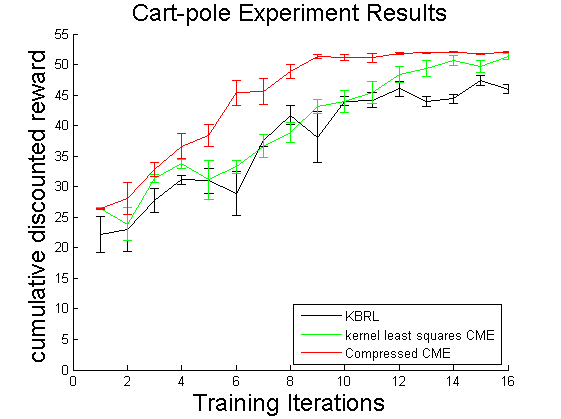
\includegraphics[width=\textwidth]{CPrewards.png}
%\caption{aaaaa}
%\label{figCPrwd}
\end{subfigure}
\begin{subfigure}[b]{0.3\textwidth}
%\centering
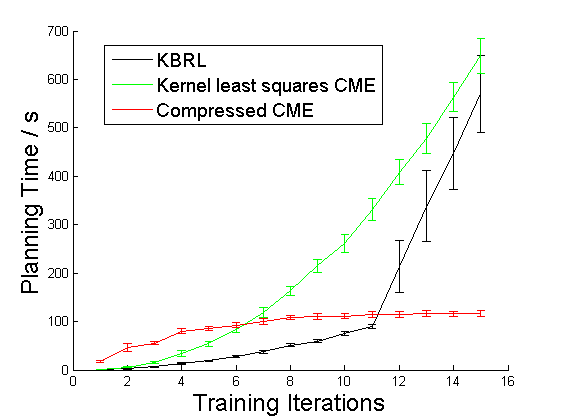
\includegraphics[width=\textwidth]{CPplanning.png}
%\caption{aaaa}
%\label{figCPp}
\end{subfigure}
\begin{subfigure}[b]{0.3\textwidth}
%\centering
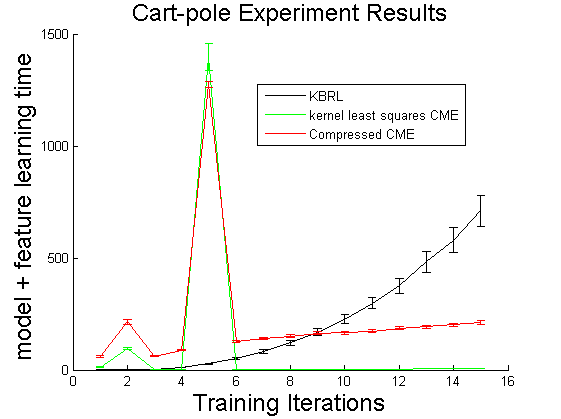
\includegraphics[width=\textwidth]{CPmodelfeature.png}
%\caption{aaaa}
%\label{figCPmf}
\end{subfigure}
\caption{Cart-pole reward and timing results}
  \label{CPfigs}
\end{figure*}

\begin{figure*}[htb]
\centering
\begin{subfigure}[b]{0.3\textwidth}
%\centering
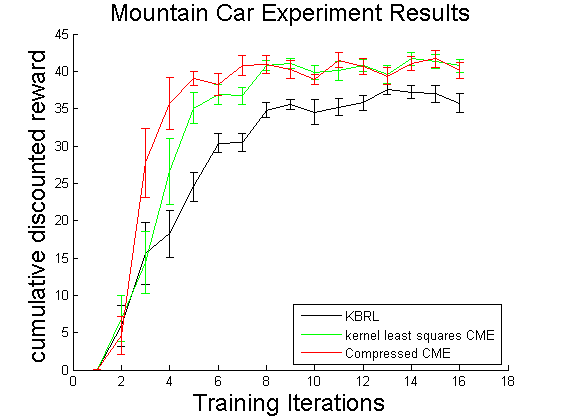
\includegraphics[width=\textwidth]{MCrewards.png}
%\caption{aaaaa}
%\label{figCPrwd}
\end{subfigure}
\begin{subfigure}[b]{0.3\textwidth}
%\centering
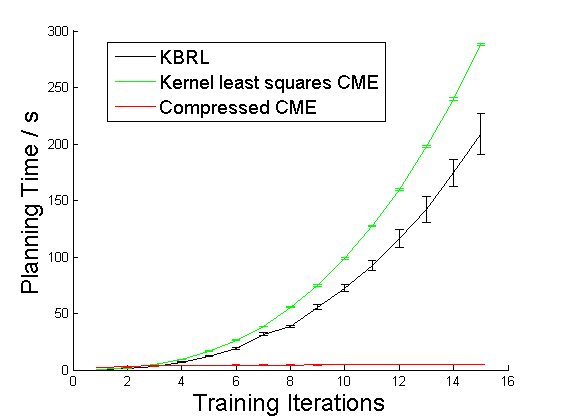
\includegraphics[width=\textwidth]{MCplanning.png}
%\caption{aaaa}
%\label{figCPp}
\end{subfigure}
\begin{subfigure}[b]{0.3\textwidth}
%\centering
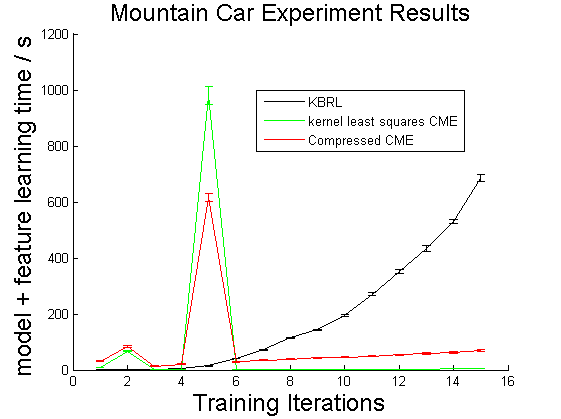
\includegraphics[width=\textwidth]{MCmodelfeature.png}
%\caption{aaaa}
%\label{figCPmf}
\end{subfigure}
\caption{Mountain-car reward and timing results}
  \label{MCfigs}
\end{figure*}


\begin{figure*}[htb]
\centering
\begin{subfigure}[b]{0.3\textwidth}
%\centering
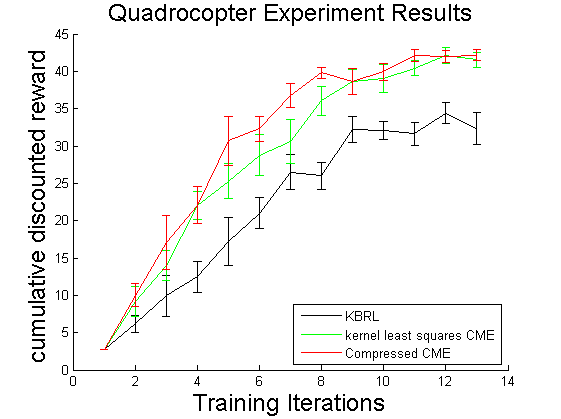
\includegraphics[width=\textwidth]{Quadrewards.png}
%\caption{aaaa}
%\label{figCPp}
\end{subfigure}
\begin{subfigure}[b]{0.3\textwidth}
%\centering
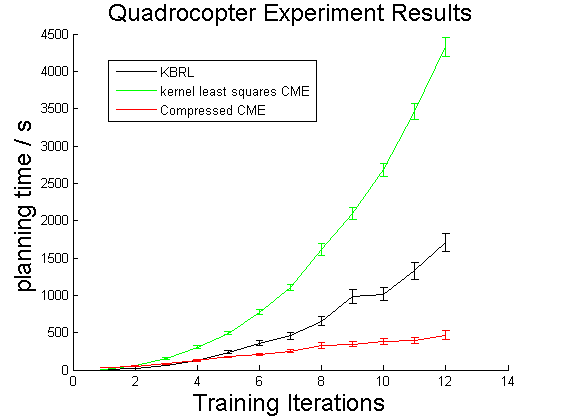
\includegraphics[width=\textwidth]{Quadplanning.png}
%\caption{aaaa}
%\label{figCPp}
\end{subfigure}
\begin{subfigure}[b]{0.3\textwidth}
%\centering
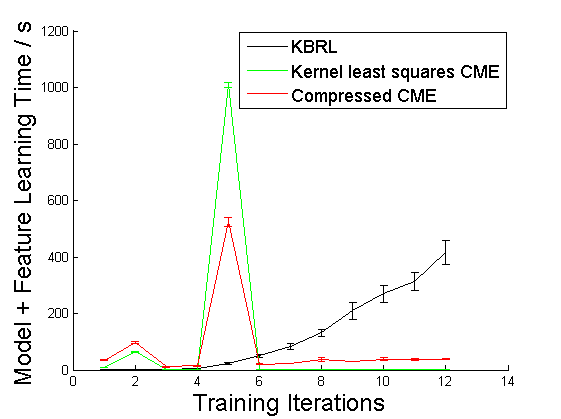
\includegraphics[width=\textwidth]{Quadmodelfeature.png}
%\caption{aaaa}
%\label{figCPmf}
\end{subfigure}
\caption{Simulated quadrocopter navigation reward and timing results}
  \label{Quadfigs}
\end{figure*}


\section{Summary}

We have presented a model-based policy iteration algorithm, based on learning a compressed CME of the transition dynamics, and solving the induced finite pseudo-MDP exactly using dynamic programming. This results in a stable algorithm with good performance guarantees in terms of the transition model error. An analysis of the CME approach suggested a principled means to choose a compression set for the CME, which guarantees an at most small loss in the representation power of the CME, and only a small degradation in performance bound. To learn the CME our approach builds a state-action representation online based on interactions with the system using sparse-greedy feature selection from a data-defined dictionary of kernel functions, enhancing the state-action representation to maximally improve the model. We overcome the planning bottleneck of competitor methods and obtain better policies on a range of MDPs. The compression approach could be used in other related algorithms such as KBRL. Future work could include using other representations of the CME in this context, such as deep neural networks. We remark that it is possible to combine the compression approach with the constrained approach of \citet{\CsabaFLAM} which we defer for a longer version.
\todoc{Other future work: Parameter sensitivity. How did we select parameters?
Other arbitrary choices:
New compression points are looked at the new data only, why?}\todog{Yes. Lets perhaps add later when we get more space.}

\appendix
\section*{Appendix}
\section{The Weight Projection via Lasso} \label{LassoSec}

Projections of the following form
\begin{align}
{\rm proj}(\balpha) = \argmin_{\bbeta \in \R^m, ||\bbeta||_1\le 1} || \sum_{j=1}^m \alpha_j \phi(s_j) - \sum_{j=1}^m \beta_j  \phi(s_j)  ||_{\cF}. \label{ProjProb}
\end{align}
are used throughout the method to maintain compression sets and project weights to obtain propoer CMEs. Problem (\ref{ProjProb}) can be reduced to:
\begin{align}
{\rm proj}(\balpha)  = \argmin_{\bbeta \in \R^m, ||\bbeta||_1\le 1} || \bR \bbeta - \bR \balpha ||_2. \nn
\end{align}
where $\bR^\top \bR = \bL$, and $L_{ij} = \lang \phi(s_i), \phi(s_j)\rang_\cF$, which can be solved with Lasso \citep{\TibshiraniLasso}. Note that the feature vectors do not need to be computed -- the Gram matrix is all that is needed. $\bR$ can be an incomplete  (low-rank) Cholesky decomposition \citep{\ShaweTaylorBook} of $\bL$ with few rows, so that the effective number of ``data points'' in the Lasso is small, and therefore efficient. For example we use an incomplete Cholesky factorization with $200$ rows in our experiments.

\section{Proof of Theorem~\ref{CompressionTheorem}} \label{learningCompressionAppendix}

We begin with a lemma:

\begin{lemma}\label{CMPlemma} Given $\{s'_1,s'_2,...,s'_n\}$, suppose $\cC = \{ c_1,...,c_m \}\subseteq \cS$ is such that for all $s'_j\in\cD$ there exists ${\bm b} = {\bm b}(s'_j)\in\R^m$, $||\bm b||_1\le 1$ such that
\begin{align}
||\sum_{i=1}^m b_i(s'_j) \phi(c_i) - \phi(s'_j)||_{\cF} \le \delta. \label{Ccondition}
\end{align}
Then let $\mu(\cdot)$ be defined via $\mu(s,a) = \sum_{j=1}^n \alpha_j(s,a) \phi(s'_j)$, with $||\balpha(s,a)||_1\le 1$ for all $(s,a)\in\cS\times\cA$. 
If we define $\alpha^{CMP}_i(s,a)=\sum_{j=1}^n b_i(s'_j) \alpha_j(s,a)$ then $\sum_{i=1}^m |\alpha^{CMP}_i(s,a)|\le 1$ and for all $(s,a)$
\begin{align}
||\mu(s,a) - \hat\mu^{CMP}(s,a)||_\cF < \delta. \nn
\end{align}
\end{lemma}

\begin{proof}
\begin{align}
\sum_{i=1}^m |\alpha^{CMP}_i(s,a)| & = \sum_{i=1}^m |\sum_{j=1}^n b_i(s'_j) \alpha_j(s,a)| \nn\\
&\le \sum_{j=1}^n|\alpha_j(s,a)| \sum_{i=1}^m  |b_i(s'_j)| \le 1, \nn
\end{align}
and,
\begin{align}
&||\hat\mu(s,a) - \hat\mu^{CMP}(s,a)||_\cF \nn\\
&= || \sum_{j=1}^n \alpha_j(s,a) \phi(s'_j) - \sum_{i=1}^m \alpha^{CMP}_i(s,a) \phi(c_i) ||_\cF \nn\\
&= || \sum_{j=1}^n \alpha_j(s,a)( \phi(s'_j) - \sum_{i=1}^m b_i(s'_j)  \phi(c_i)) ||_\cF \nn\\
&\le \sum_{j=1}^n |\alpha_j(s,a)| \max_j || \phi(s'_j) - \sum_{i=1}^m b_i(s'_j)  \phi(c_i)) ||_\cF\nn\\
&\le \delta.\nn
\end{align}
\end{proof}

Note that by construction the compression set returned by Algorithm~\ref{CompressionRoutine} satisfies condition (\ref{Ccondition}) and is therefore a $\delta$-lossy compression. Hence Lemma~\ref{CMPlemma} directly implies Theorem~\ref{CompressionTheorem}.


\section{Experimental Details} \label{ExperimentDetails}

We here give more details of the experiments for reproducibility purposes. We begin with settings common to all MDPs. The horizon of each MDP is 100, so that $n_{\rm new} = 200$ data points were added at each iteration. To perform planning at each iteration we performed $J=10$ policy evaluation/improvement steps, before returning to the MDP to collect more data. For the compressed CME the size of the sparse-greedy feature space was constrained to be no greater than $d=200$. For all 3 methods we performed 5-fold cross-validation over 10 bandwidth parameters to optimize the ``input'' kernel $K$ on $\cS\times\cA$. For the two least-squares methods we also cross-validated the regularization parameter over 20 values. The ``output'' feature map $\phi(\cdot)$ also corresponds to a Gaussian kernel $\phi(s) = L(s,\cdot)$, and the bandwidth of $L$ was chosen using an informal search for each MDP (it is not clear how this parameter can be validated during the algorithm). For planning we set $\gamma=0.98$, but we report results for $\gamma=0.99$. \todoc{Why? This is weird and calls for an explanation.}\todog{Yes sorry this is just a legacy from previous code where LSTD is better with smaller $\gamma$. Really there are two $\gamma$s if you like, one defined by an MDP and the other is a parameter of the algorithm. You get faster contractions with smaller $\gamma$ but since we invert anyway it probably doesn't make any difference here to switch. For a final version I'll rerun with $\gamma=0.99$.}
\todoc{Add how we measured the cumulated discounted rewards on the figures: freezing the policies, running them from $P_1$.}

\subsection{Cart-Pole Experiment Details}

This problem simulates a pole attached at a pivot to a cart, and by applying force to the cart the pole must be swung to the vertical position and balanced. The problem is under-actuated in the sense that insufficient power is available to drive the pole directly to the vertical position, hence the problem captures the notion of trading off immediate reward for long term gain. We used the same simulator as \citet{DBLP:journals/jmlr/LagoudakisP03}, except here we choose a continuous reward signal. The state space is two dimensional, $s = (\theta, \dot{\theta})$ representing the angle ($\theta = 0$ when the pole is pointing vertically upwards) and angular velocity of the pole. The action set is $\{-50,0,50\}$ representing the horizontal force in Newtons applied to the cart. Uniform noise in $[-10,10]$ is added to each action. The system dynamics are $\theta_{t+1} = \theta_t + \Delta_t \dot {\theta_t}$, $\dot\theta_{t+1} = \dot\theta_t + \Delta_t \ddot {\theta_t}$ where
$$ \ddot {\theta} = \frac{g \sin(\theta) - \alpha m \ell (\dot{\theta})^2 \sin(2 \theta)/2 - \alpha \cos(\theta) u}{ 4\ell / 3 - \alpha m \ell \cos^2(\theta)}, $$
where $g=9.8m/s^2$ is the acceleration due to gravity, $m=2kg$ is the mass of the pole, $M = 8kg$ is the mass of the cart, $\ell = 0.5m$ is the length of the pole and $\alpha = 1/(m+M)$. We choose $\Delta_t = 0.1s$. Rewards $R(s,a) = \frac{1+ \cos(\theta)}{2}$, the discount factor is $\gamma = 0.99$, the horizon is $H=100$, and the pole begins in the downwards position, $s_0 = (\pi,0)$.

The state kernel is a Gaussian $L(s,s') = \exp\left({\frac{1}{2\sigma_{\cS}^2}(s - s')^\top \bM_\cS (s - s')}\right)$ with $\bM_\cS =\left( \begin{array}{cc}
1 & 0 \\
0 & 1/4 \end{array} \right)$, and the state-action kernel is  $K((s,a),(s',a')) = \exp\left({\frac{1}{2\sigma_{\cS\times\cA}^2}((s,a) - (s',a'))^\top \bM_{\cS\times\cA} ((s,a) - (s',a'))}\right)$ with
$$\bM_{\cS\times\cA} =\left( \begin{array}{ccc}
1 & 0 & 0\\
0 & 1/4 & 0\\
0 & 0 & 1/10000 \end{array} \right).$$ The output feature map $\phi(s) = L(s,\cdot)$ with $\sigma_{\cS} = 0.5$ (chosen by informal search). During model learning we performed 5-fold cross validation over a range of 10 bandwidths in the range $[0.01,5]$ to optimize $\sigma_{\cS\times\cA}$. For the compressed CME the tolerance of the compression set selection was set to $\delta = 0.1$, i.e. we use a $\delta$-lossy compression set $\cC$ with $\delta=0.1$.

Cumulative reward of 50 is a near optimal policy in which the pole is quickly swung up and balanced for the entire episode. Cumulative reward of 40 to 45 indicates that the pole is swung up and balanced, but either not optimally quickly, or that the controller is unable to balance the pole for the entire remainder of the episode. 

\subsection{Mountain-Car Experiment Details}

In this problem the agent controls a car located at the bottom of a valley and the objective is to drive to the top of a hill but does not have enough power to achieve this directly and must climb the opposite hill a short distance before accelerating toward the goal (see e.g. \citet{\SinghEligibility}). States $s =(x,v)$ are position and velocity, $\cS=(-1.2,0.7)\times(-0.07,0.07)$, $\cA=\{-1,0,1\}$ and $r(s,a) = e^{-8(x-0.6)^2} $ and $s_0 = (-0.5,0)$. Dynamics are $x' = x+v+\epsilon_1$, $v' = v + 0.001a -0.0025 \cos(3 x) + \epsilon_2/10$, where $\epsilon_1, \epsilon_2$ are Gaussian random variables with standard deviation $0.02$. If $x'>0.6$ then the state is set to $(0.6,0)$. For a horizon $H=100$ the optimal return is around 45. Doing nothing receives almost no reward. 

The state kernel is a Gaussian $L(s,s') = \exp\left({\frac{1}{2\sigma_{\cS}^2}(s - s')^\top \bM_\cS (s - s')}\right)$ with $\bM_\cS =\left( \begin{array}{cc}
1 & 0 \\
0 & 1/100  \end{array} \right)$, and the state-action kernel is  $K((s,a),(s',a')) = \exp\left({\frac{1}{2\sigma_{\cS\times\cA}^2}((s,a) - (s',a'))^\top \bM_{\cS\times\cA} ((s,a) - (s',a'))}\right)$ with
$$\bM_{\cS\times\cA} =\left( \begin{array}{ccc}
1 & 0 & 0\\
0 & 1/100 & 0\\
0 & 0 & 1/25\end{array} \right).$$ The output feature map $\phi(s) = L(s,\cdot)$ with $\sigma_{\cS} = 0.5$ (chosen by informal search). During model learning we performed 5-fold cross validation over a range of 10 bandwidths in the range $[0.01,5]$ to optimize $\sigma_{\cS\times\cA}$. For the compressed CME the tolerance of the compression set selection was set to $\delta = 0.01$, i.e. we use a $\delta$-lossy compression set $\cC$ with $\delta=0.01$.




\subsection{Quadrocopter Experiment Details}

The state kernel is a Gaussian $L(s,s') = \exp\left({\frac{1}{2\sigma_{\cS}^2}(s - s')^\top \bM_\cS (s - s')}\right)$ with $\bM_\cS =diag( \bone/25, \bzero ,\bone, \bzero ,0)$ where $\bone = (1,1,1)$, $\bzero = (0,0,0)$ (which essentially reduces the state observations to 6 dimensions), and the state-action kernel is
\begin{align}
&K((s,a),(s',a')) \nn\\
&= \hspace{-0.5mm}\exp\hspace{-0.8mm}\left({\frac{1}{2\sigma_{\cS\times\cA}^2}((s,a)\hspace{-0.8mm} - \hspace{-0.8mm}(s',a'))^\top \hspace{-0.5mm}\bM_{\cS\times\cA} ((s,a)\hspace{-0.8mm} -\hspace{-0.8mm} (s',a'))}\right)\nn
\end{align}
with $\bM_{\cS\times\cA} =diag(\bone /25,\bzero ,\bone,\bzero,0,  \bone/100)$. The output feature map $\phi(s) = L(s,\cdot)$ with $\sigma_{\cS} = 1$ (chosen by informal search). During model learning we performed 5-fold cross validation over a range of 10 bandwidths in the range $[0.01,5]$ to optimize $\sigma_{\cS\times\cA}$. For the compressed CME the tolerance of the compression set selection was set to $\delta = 0.1$, i.e. we use a $\delta$-lossy compression set $\cC$ with $\delta=0.1$.



%\clearpage
%\begin{small}
\fontsize{9.5pt}{10.5pt} \selectfont
\bibliographystyle{aaai}
\bibliography{cme4mdp}
%\bibliographystyle{apalike}
%\bibliographystyle{abbrv}
%\end{small}
\fontsize{10pt}{12pt} \selectfont

\clearpage



\section{Additional Details of the Feature Selection Process}\label{MatchingPursuit}

\subsection{Sparse-Greedy Regression with Vector-Valued Matching Pursuit}

Our algorithm uses, as a subcomponent, a vector-valued version of the matching pursuit algorithm \citep{\MallatMatchingPursuit}. The use of matching pursuit for vector-valued regression is not new \citep{\LeverPoliciesInRKHS} but we provide details for completeness. This adaptation can handle targets in general vector spaces $\cV$. Since the algorithm only computes inner products between vectors in the target space $\cV$ it can be kernelized, i.e. we can learn an RKHS-valued function. This is a straightforward extension of the scalar case, we derive the method here for clarity.

Suppose we wish to regress a vector-valued function
\begin{align}
f^*:\cX\to\cV, \nn
\end{align}
given a data sample $\cD = \{x_i,v_i\}_{i=1}^m$ where $v_i = f^*(x_i)+\epsilon$ where $\epsilon$ is zero-mean noise, $f^*(x_i) = \E[V_i|x_i]$. Suppose we are given a \emph{dictionary} $\cG = \{g_1,...,g_n\}$, where $g_i:\cX\to\R$, of candidate real-valued functions, and we aim to find an estimate $\hat f$ for $f^*$ of the form,
\begin{align}
\hat f = \sum_{i=1}^D w^i \hat g_i \nn
\end{align}
where $\cB_D = \{ \hat g_i \}_{i=1}^D \subseteq \cG$ is called the basis and $w^i\in\cV$. When $\cV=\R$, matching pursuit \citep{\MallatMatchingPursuit} can be used to incrementally build the basis, and we now detail the extension to the vector-valued output case. We build the basis incrementally and for each basis $\cB_j$ we form an estimate $\hat f^j = \sum_{i=1}^j w^i \hat g_i$. We begin with the empty basis $\cB_0$  and add new basis elements $\hat g_{j+1}$ to greedily optimize the objective. For each estimate we define the residue $\br^j$,
\begin{align}
r^j_i = v_i - \hat f_j(x_i) \in\cV , \nn
\end{align}
and pick the $g\in\cD$ which minimizes the next residue when added to the current estimate,
\begin{align}
g_{j+1} &= \argmin_{g\in\cD}\min_{w \in\cV} \sum_{i=1}^m ||v_i - ( (\hat f_j + w g) (x_i)  )||_{\cV}^2 \nn\\
&=\argmin_{g\in\cD}\min_{w\in\cV} \sum_{i=1}^m ||r^j_i -  w g(x_i)  ||_{\cV}^2. \nn
\end{align}
Since $\nabla_{w}  \sum_{i=1}^m ||r^j_i -  w g(x_i)  ||_\cV^2  = 0$ at the minimum we have,
\begin{align}
0 &= \sum_{i=1}^m  \nabla_w \left(  \lang  g(x_i)w,g(x_i)w  \rang_{\cV} -2\lang g(x_i) w, r^j_i \rang_\cV \right)  \nn\\
&=  \sum_{i=1}^m 2w g(x_i)^2 -2 g(x_i)  r^j_i  \nn\\
w^{j+1} &=  \left(\sum_{i=1}^m  g(x_i)  r^j_i \right) /\left( \sum_{i=1}^m  g(x_i)^2 \right) \in\cV \nn
\end{align}
Then,
\begin{align}
&\sum_{i=1}^m ||r^j_i -  w^{j+1} g(x_i)  ||_{\cV}^2 \nn\\
&=  \sum_{i=1}^m ||r^j_i||_\cV^2 - 2\sum_{i=1}^m g(x_i)\lang  r^j_i,w^{\rm min} \rang_\cV \nn\\
&\quad + ||w^{\rm min}||_\cV^2 \sum_{i=1}^m  g(x_i)^2 \nn\\
&= \sum_{i=1}^m ||r^j_i||_\cV^2 - \frac{2\sum_{i=1}^m g(x_i)\lang  r^j_i, \sum_{k=1}^m  g(x_k)  r^j_k   \rang_\cV}{ \sum_{k=1}^m  g(x_k)^2} \\
&\quad + \frac{ ||\sum_{k=1}^m  g(x_k)  r^j_k  ||_\cV^2 }{ \sum_{i=1}^m  g(x_i)^2 }\nn\\
&= \sum_{i=1}^m ||r^j_i||_\cV^2 - \frac{ ||\sum_{i=1}^m  g(x_i)  r^j_i  ||_\cV^2 }{ \sum_{i=1}^m  g(x_i)^2 }\nn
\end{align}
Thus $\hat g_{j+1} = \argmax_{g\in\cG}  \frac{ ||\sum_{i=1}^m  g(x_i)  r^j_i  ||_\cV^2 }{ \sum_{i=1}^m  g(x_i)^2 }$. Thus at each iteration of matching pursuit we must evaluate $\frac{ ||\sum_{i=1}^m  g(x_i)  r^j_i  ||_\cV^2 }{ \sum_{i=1}^m  g(x_i)^2 }$ for a selection of $k$ dictionary elements (not necessarily all). We have,
\begin{align}
 ||\sum_{i=1}^m  g(x_i)  r^j_i  ||_\cV^2  &=  ||\sum_{i=1}^m  g(x_i) (\hat f^j(x_i) - v_i)  ||_\cV^2 \nn
\end{align}
For each dictionary element $g$ this can be computed in $O(mj+md+jd)$ where $d={\rm dim}(\cV)$, and so $O(k(mj+md+jd))$ over $k$ dictionary elements.

It is sometimes useful, at iteration $j$ to ``backfit'' all the weights $\{w^i\}_{i=1}^j$ by replacing them with the least squares solution: i.e. matching pursuit is used to find the basis but the weights are finally optimized using least squares. Alternatively this can be performed end of the process or several times throughout.

In order to find a compact representation we can also use matching pursuit adaptively by setting a tolerance $\delta$ such that the algorithm terminates when it fails to reduce the residue by more than $\delta$. Thus the method will only add features if they significantly reduces the objective.

The output of vector valued matching pursuit is a collection of weights $\{w^i\}_{i=1}^j$ and features $\{ \hat g_i(\cdot) \}_{i=1}^j$ such that $f^* \approx \sum_{i=1}^j w^i \hat g_i$. 


\subsubsection{Fast Feature Selection For RKHS-Valued Matching Pursuit}

Performing matching pursuit to regress a function $f:\cS\times\cA\to\cF_L$ where $\cF_L$ is an RKHS whose feature map $\phi(s)=L(s,\cdot)$ is high- or even infinite-dimensional can become expensive when the number of data points becomes large. This is because the expansion of each target residue for matching pursuit will have an expansion in the RKHS $\cF_L$ in the number of data points, and so computing a single inner product scales with the size of the data, and feature selection by this method would be the bottleneck in Algorithm~\ref{PIwCMEfeatures}. To solve this problem we map the target data for matching pursuit, i.e. the residues $\cR(s_i,a_i,s_i')\in\cF_L$ for $(s_i,a_i,s'_i)\in\cD$, into a lower dimensional subspace of $\cF_L$ using an incomplete Cholesky decomposition of the kernel matrix $\bL$ \citep{\ShaweTaylorBook}. This provides an approximation $\bL \approx \bR^\top \bR$ of the $n\times n$ matrix $\bL$ where $\bR$ is a $p\times n$ matrix $\bR = ( \br_1,...,\br_n)^\top$, where $p\ll n$ can be chosen or chosen adaptively using a tolerance parameter. This approximation is often excellent \citep{\BachLowRank} and captures the inner products in $\cF_L$ since $\br_i^\top \br_j \approx L_{ij} = \lang \phi(s'_i), \phi(s'_j)\rang_L$, thus we can ``project'' the high-dimensional feature vectors $\phi(s'_i)$ to $\R^p$ via $\phi(s'_i)\mapsto \br_i$, approximately preserving inner products. We then have the following approximation for the loss function,
\begin{align}
\widehat\loss_{\lambda}(\bW) &= \frac{1}{n}\sum_{i=1}^n ||\sum_{j=1}^n \psi(s_i,a_i)^\top \bw_j\phi(s_j) - \phi(s_i) ||^2_\cF \nn\\
&\approx \frac{1}{n}\sum_{i=1}^n ||\sum_{j=1}^n \psi(s_i,a_i)^\top \bw_j\br^\top_j - \br^\top _i ||^2
\end{align}
Thus if we define the following ``projection'' of the model residues
\begin{align}
\bq_i&:= \br^\top _i - \sum_{j= 1}^{n_k} \psi^k(s_i,a_i)^\top  \bw^j_{k}\br^\top _j \in \R^p, \label{ProjectedResidues}
\end{align}
and we perform vector-valued matching pursuit using the approximate, low dimensional residue data $\{(s_i,a_i),\bq_i\}_{i=1}^n$ in $p$-dimensional Euclidean space we will find find a feature $\psi^{\rm new}(\cdot)$ and a weight $\bbb^{\rm new} = \sum_{j=1}^n w_j^{\rm new} \br_j^\top$ such that
\begin{align}
\sum_{i=1}^n ||\psi^{\rm new}(s_i,a_i)^\top \bbb^{\rm new}+ \sum_{j=1}^n \psi(s_i,a_i)^\top \bw_j\br^\top_j - \br^\top _i ||^2 \nn
\end{align}
is minimized w.r.t $\psi^{\rm new}(\cdot)\in\cG$ and $\bbb^{\rm new}\in\R^p$. But then $\psi^{\rm new}(\cdot)$ and a $b^{\rm new} := \sum_{j=1}^n w_j^{\rm new} \phi(s'_j)$ are (approximately) optimally greedy for $\widehat\loss_{\lambda}(\bW)$ in the sense that
\begin{align}
\sum_{i=1}^n\hspace{-0.6mm} || \psi^{\rm new}(s_i,a_i)^\top b^{\rm new} \hspace{-0.6mm} +\hspace{-0.6mm} \sum_{j=1}^n\hspace{-0.6mm} \psi(s_i,a_i)^\top \bw_j\phi(s_j)\hspace{-0.6mm} - \hspace{-0.6mm}\phi(s_i) ||^2_\cF \nn
\end{align}
is minimized w.r.t. $\psi^{\rm new}(\cdot)\in\cG$ and $b^{\rm new}\in\cF$. i.e. performing matching pursuit on the low dimensional residues is an equivalent problem up to approximation error of the Cholesky decomposition and the same features will be returned if this decomposition is accurate.  In this way $d_{\rm new}$ new features can be added in time $O(d_{\rm new} p|\cG||\cD|)$, where $p$ is the rank of the incomplete Cholesky decomposition. In our experiments $p$ was set to $p=200$ by computational budget and the kernel approximation was found to be almost perfect.

\iffalse
Essentially the method finds a low-dimensional subspace of $\cF_L$, spanned by $n$ representative points which are greedily selected, on which most of the feature-mapped data points approximately reside. The application to RL is interesting since data may accumulate in certain regions of the state space, hence it is often possible to obtain a small set of good representative points and the Cholesky approach provides principled, fast means of finding the low dimensional representation. 

Note that if we had not retained the loss function of \citet{\GrunewalderEmbeddingsRL} we would not be able to perform efficient feature selection in this way since the ``kernel matrix'' we would need to perform an incomplete Cholesky decomposition would be an identity matrix, and there would be no sensible low rank approximation. Equivalently each data point is mapped into feature which is perpendicular to all other data features, and so no low dimensional subspace can explain the feature mapped data.
\fi




\iffalse


\section{Solving the Constrained Compressed CME problem with ADMM **needs updating**}\label{ConstCompSol}

We now investigate the possibility of applying the constrained optimization approach of \citet{\CsabaFLAM} to the more general loss function of \citet{\GrunewalderEmbeddingsRL}, which admits general feature maps $\phi(\cdot)$, to obtain the ``best of both worlds''. Thus we are interested in minimizing:
\begin{align}
\widehat\loss_{\lambda}(\bW) = \frac{1}{n} || \bPsi \bW - \bI ||^2_{Fr(\bL)} + \lambda||\bW||^2_{Fr(\bL)}, \nn
\end{align}
subject to the constraint
$$||\psi(s'_i,a)^\top \bW||_1\le 1  \quad \quad \mbox{ for all } i\le n \mbox{ and } a\in\cA. $$
This is possible, and we present the method in a more general context, with additional compression of the CME.

First of all we note that the solution to the unconstrained case is $\bW = (\bPsi^\top \bPsi + \lambda \bI)^{-1} \bPsi^\top \bL_{\cD\cC}\bL_{\cC\cC}^{-1}$ which can be seen by differentiating the unconstrained objective. For the constrained case we form the augmented Lagrangian,
\begin{align}
&\cL_\rho(\bW,\bY,\bLambda) = \frac{1}{n} \trace\left( \bPsi \bW \bL_{\cC\cC} \bW^\top \bPsi^\top - 2\bPsi\bW\bL_{\cC\cD}  \right) \nn\\
&\quad + \lambda  \trace\left(\bW \bL_{\cC\cC} \bW^\top\right) + \delta\left( ||\bY||_{1,\infty} \le 1 \right) + \rho||\bY-\bA^\top\bW-\bLambda||^2_{Fr}, \label{AugmentedLagrangian}
\end{align}
where $\delta(\cE)$ is the indicator of event $\cE$. A generic ADMM procedure \citep{\BoydADMM} for minimizing the Lagrangian (\ref{AugmentedLagrangian}) is given in Algorithm~\ref{ADMM}.\footnote{**There are several options here. I am using the ``scaled form'' and there is a choice in the order in which we do the steps. Does it matter?**}\begin{algorithm}[tb]
   \caption{ADMM for solving the constrained compressed CME}
   \label{ADMM}
\begin{algorithmic}
	 \STATE {\bf Initialize:} $\bW_0 = (\bPsi^\top \bPsi + \lambda \bI)^{-1} \bPsi^\top \bL_{\cD\cC}\bL_{\cC\cC}^{-1}$ (unconstrained minimizer\footnote{**Numerical issues with the inverse?**}), $\rho = 1$,\footnote{**How to choose?**} $\bY_0 = \bA^\top \bW_0$, $\bLambda_0 = \bZero$.
	 \FOR {$t=1,2,...$}
	 \STATE {\bf Step 1:} $\bW_t = \argmin_{\bW} \cL_\rho(\bW,\bY_{t-1},\bLambda_{t-1})$\\
	 \STATE {\bf Step 2:} $\bY_t = \argmin_{\bY} \cL_\rho(\bW_t,\bY,\bLambda_{t-1})$ \\
   \STATE {\bf Step 3:} $\bLambda_t = \bLambda_{t-1} + \bA^\top\bW_t - \bY_t$ \\
	 \ENDFOR
\end{algorithmic}
\end{algorithm}

We discuss the steps in turn:

\underline{\bf Step 1:} Setting $\nabla_{\bW} \cL(\bW,\bY,\bLambda) = 0$ gives:
\begin{align}
 \frac{1}{n}(\bPsi^\top \bPsi \bW \bL_{\cC\cC} - \Psi^\top\bL_{\cD\cC}) + \lambda\bW\bL_{\cC\cC}  &= \rho\bA(\bY-\bA^\top\bW-\bLambda) \nn\\
(\bPsi^\top \bPsi + n\lambda\bI)\bW \bL_{\cC\cC} + n\rho \bA\bA^\top\bW &= \bPsi^\top\bL_{\cD\cC} + n\rho\bA\bY - n\rho\bA\bLambda\nn\\
(\bPsi^\top \bPsi + n\lambda\bI)^{-1}n\rho \bA\bA^\top \bW + \bW \bL_{\cC\cC} &= (\bPsi^\top \bPsi + n\lambda\bI)^{-1}(\bPsi^\top\bL_{\cD\cC} + n\rho\bA\bY - n\rho\bA\bLambda)
\end{align}
This is a Sylvester equation and, once the matrices $(\bPsi^\top \bPsi + n\lambda\bI)^{-1}n\rho \bA\bA^\top$ and $(\bPsi^\top \bPsi + n\lambda\bI)^{-1}(\bPsi^\top\bL_{\cD\cC} + n\rho\bA\bY - n\rho\bA\bLambda)$ have been computed, can be solved in time $d^3+m^3$ (i.e. the bottleneck is likely to be constructing the required matrices, rather than solving the equation).\footnote{**Need to check this. Matlab routines exist. Are there numerical issues?**} Setting $\bL_{\cC\cC} = \bL_{\cD\cC} = \bI$, $\lambda= 0$ recovers the method of \citet{\CsabaFLAM} for the special case considered therein\footnote{**There is a change of notation required: $\bW \rightarrow \bF^\top$, $n\rho \rightarrow \frac{1}{\mu}$.**}.

\underline{\bf Step 2:} is a Euclidean projection to the $L_1$ unit ball and can be solved using the method of \citet{\DuchiProjections}, exactly as in as in \citet{\CsabaFLAM}.

\underline{\bf Step 3:} is trivial.

\subsection{Possible Problems}

We may wish to avoid the Sylvester equation in favor of a closed form solution for step 1. This seems possible if we adopt a slightly different augmented Lagrangian (which may be more sensible since the penalty is taken in the RKHS norm):
\begin{align}
&\cL_\rho(\bW,\bY,\bLambda) = \frac{1}{n} \trace\left( \bPsi \bW \bL_{\cC\cC} \bW^\top \bPsi^\top - 2\bPsi\bW\bL_{\cC\cD}  \right)  + \lambda   \trace\left(\bW \bL_{\cC\cC} \bW^\top\right)\nn\\
&\quad + \rho||\bY-\bA^\top\bW||^2_{Fr(\bL_{\cC\cC})} - \trace(\bLambda^\top(\bY - \bA^\top\bW))+ \delta\left( ||\bY||_{1,\infty} \le 1 \right) , \label{AugmentedLagrangian2}
\end{align}
but in this case the projection of step 2 is not a Euclidean projection, but a projection w.r.t. $||\bx||^2_{\bL_{\cC\cC}} = \bx^\top\bL_{\cC\cC} \bx$.\footnote{**I guess this is just as easy but a little bit of work would have to be done to use the standard projection.**}




\section{Orphans}

\subsection{Constructing the Feature Dictionary}

We define the dictionary $\cG_k$ adaptively at each stage, in a data-driven way. Given a kernel $K$ on $\cS\times\cA$, when encountering some transitions $\{(s_i,a_i,s'_i)\}_{i=1}^{n_{\rm new}}$ during exploration at round $k$, we set $\cG_k = \{g_i(\cdot) = K((s_i,a_i),\cdot)\}_{i=1}^{n_{\rm new}}$, as in kernel matching pursuit \citep{\BengioKernelMP}, in which case we will learn an estimator $\hat\mu(s,a) = \sum_{ij=1}^{n} \phi(s'_i) W_{ij} K((s_j,a_j),(s,a))$ which has the form of a kernel regressor, but here matching pursuit will ensure that the size of this expansion is controlled by only incorporating useful features (most columns of $\bW$ will be zero). We use Gaussian kernels in our experiments. The approach is general and the dictionary could include arbitrary real-valued functions, including, for example, those used by unsupervised learning methods.



\subsection{Online Model Updates Using  Matching Pursuit} \label{OnlineModelUpdate}

It may be of interest to update the model in a faster incremental fashion rather than via the full relearn of (\ref{ModelUpdateFormula}), since Matching pursuit returns weights as well as features, this can be achieved and we detail the procedure here. Note that, for $\theta_k\in[0,1]$,
\begin{align}
\sum_{(s,a,s')\in\cD_k} || \cR(s,a,s') - \theta_k \hat\cR(s,a) ||^2_{\cF} \le  \sum_{(s,a,s')\in\hat\cD_k} || \cR(s,a,s') ||^2_{\cF}, \nn
\end{align}
since matching pursuit only adds features $\hat g_j(\cdot)\in\cG_k$ and weights $b_j\in\cF$ if they reduce the objective (\ref{MPObjective}). It is the case that
\begin{align}
(b_1, b_2,...,b_\ell)^\top = \bW_{\rm new} \bPhi_{k}
\end{align}
for some matrix $\bW_{\rm new}$. Therefore setting $\bW^\top_k =  \left( \begin{array}{cc}
 \bW_{k-1} &  \bzero  \\
\theta_k \bW_{\rm new} \end{array} \right)$,  where $\theta_k\in[0,1]$ is a learning rate, we have that
$\psi^k(s,a)^\top\hat\bW_k \bPhi_k =  \psi^{k-1}(s,a)^\top\hat\bW_{k-1}\bPhi_{k-1} + \theta_k \psi^{\rm new}(s,a)^\top \bW_{\rm new}\bPhi_k$, and therefore,
\begin{align}
\sum_{(s,a,s')\in\cD_k} || \phi(s') -\psi^k(s,a)^\top\bW_k \bPhi_k  ||^2_{\cF} &=\sum_{(s,a,s')\in\cD_k} || \cR(s,a,s') - \theta_k \hat\cR(s,a) ||^2_{\cH}\nn\\
&\le \sum_{(s,a,s')\in\cD_k} || \phi(s') -  \psi^{k-1}(s,a)^\top\bW_{k-1} \bPhi_{k-1}||^2_{\cF} \nn
\end{align}
i.e. the empirical loss of the model is reduced (on $\cD_k$) by the addition of new weights and features. In practice the new matrix component $\bW_{\rm new}$ would be ``backfitted'' i.e. relearned by linear least-squares regression to fit the residue targets $\cR(s,a,s')$ on $(s,a)$ over the data (or a minibatch) using the new features $\psi^{\rm new}(\cdot)$. Since the increments $\psi^{\rm new}(\cdot)$ is a very low dimensional feature map this is closed form and fast.





\subsection{Sparse-Greedy CMEs for RL using Kernel Matching Pursuit} \label{FeatureLearning}

A key problem with the existing approaches discussed in Section~\ref{learningCMEs} is their ability to maintain a compact representation of state-actions suitable for the problem. In \citet{\GrunewalderEmbeddingsRL} a rich representation is possible since the non-parametric kernel regressor has an expansion on all data, but model learning therefore scales poorly with the data size. In \citet{\CsabaFLAM} a suitable compact model is assumed to be provided a-priori the learning process which is unrealistic in most practical problems.

We now propose a method to incrementally construct a compact feature map $\psi(\cdot)$ on state-actions during policy optimization, in a data-driven way, essentially co-optimizing the feature representation and the model. The resulting representation will enable fast model learning, but in a rich space due to the adaptive nature of the state-action representation. Our approach uses a variant of the matching pursuit algorithm \citep{\MallatMatchingPursuit}, which is a principled and efficient sparse greedy approach to feature selection \citep{\ZhangMPConsistencey,\HussainTheoryOfMP}.

Our loss function for \emph{features} will be as in (\ref{GFLoss})
\begin{align}
\widehat\loss_{\lambda}(\bW) &= \frac{1}{n}\sum_{i=1}^n ||\sum_{j=1}^d\sum_{k=1}^n \psi_j(s_i,a_i) W_{jk}\phi(s'_k) - \phi(s'_i) ||^2_\cF\nn
\end{align}
i.e. we will pick features to maximally improve this loss. Suppose we have $n$ datapoints $\cD=\{s_i,a_i,s'_i\}_{i=1}^n$ and have the current feature map $\psi:\cS\times\cA\to\R^d$ and the model $\hat \mu(s,a) = \psi(s,a)^\top\bW\bPhi$. Let $\cG = \{ g_1(\cdot), g_2(\cdot),...\}$ be a dictionary of candidate functions, where each $g_j:\cS\times\cA\to\R$. We select new feature components $\psi_j(\cdot)$ greedily from $\cG$, in order to improve the dynamics model as follows. We define the \emph{model residue} $\cR:\cS\times\cA\to\cH$ of $(\psi,\bW)$ by
\begin{align}
\cR(s,a,s'):= \phi(s') - \psi(s,a)^\top\bW\bPhi  \in \cF, \label{ResidueDef}
\end{align}
for each $(s,a,s') \in \hat\cD$ where $\bPhi:=\left( \phi(s_1'),..., \phi(s'_n) \right)^\top$ which should be interpreted as a vector of functions when $\cF_L$ is an RKHS. We then use matching pursuit to regress the model residue (\ref{ResidueDef}) by selecting a small set of features $\{ \hat g_1(\cdot),...,\hat g_{d_{\rm new}}(\cdot) \} \subseteq\cG$ and weights $\{b_j \in\cF\}_{j=1}^{d_{\rm new}}$ such that $\hat\cR(\cdot) := \sum_{j=1}^{d_{\rm new}} b_j \hat g_j(\cdot) $ approximates the residue $\cR(\cdot)$ by fitting on the data $\cD$ (or a minibatch if $|\cD|$ is large),
\begin{align}
{\rm err}( \hat\cR ):=\sum_{(s,a,s')\in\cD} || \cR(s,a,s') -  \sum_{j=1}^{d_{\rm new}} b_j \hat g_j(s,a)  ||^2_{\cF}. \label{MPObjective} 
\end{align}
This is achieved by optimizing sequentially over single features and weights, adding a new feature to maximally reduce (\ref{MPObjective}) each time, until the residue cannot be significantly reduced further. We then set $\psi_i^{\rm  new}(\cdot):= \hat g_i(\cdot)$, augmenting the feature representation $\psi(\cdot) \leftarrow \left( \begin{array}{c}
\psi(\cdot) \\
\psi^{\rm new}(\cdot) \end{array} \right)$. The number $d_{\rm new}$ of features added is chosen by validating the regressors $\hat\cR(\cdot) := \sum_{j=1}^\ell b_j \hat g_j(\cdot)$ produced, for each $\ell$, on a held out set of residue data. Once the new feature map is obtained we relearn the dynamics model by regularized least squares on all available data, i.e. set $\bPsi = \left( \psi(s_1,a_1),...,\psi(s_n,a_n) \right)$ and update the model via,
\begin{align}
\bW = (\bPsi^\top \bPsi + \lambda n\bI)^{-1}\bPsi^\top \label{ModelUpdateFormula}
\end{align}
where $\lambda$ is validated using a hold out set. This is fast since the inversion is of a $d\times d$ matrix, but for very large problems it may be of interest to update the model online, as we discuss in Appendix~\ref{OnlineModelUpdate}. Since each new feature was added in order to maximally fit the model residue, this is equivalent to greedily reducing the model error, per feature. i.e. we co-optimize the state-action feature representation and the model by incrementally adding features to improve the model loss. In practice, after every round of feature augmentation, we sparsify our current feature map by applying matching pursuit to the current feature set to ensure we maintain as compact a set of features as possible.

Since the model residue targets that we regress using matching pursuit are not real numbers but RKHS functions we need a version of the matching pursuit algorithm for the case when the targets are in general vector spaces. It is possible to perform matching pursuit in general Hilbert-space-valued regression problems since only inner products between targets, rather than the targets themselves need to be evaluated. This version of matching pursuit is detailed in Appendix~\ref{MatchingPursuit}. 






\subsection{Learning Linear CMEs for RL} \label{LinearCME}

Let us suppose that a good state-action representation $\psi:\cS\times\cA\to \cH$ is available, where $\cH$ is a feature space (in Section~\ref{FeatureLearning} we will propose a method to learn such a representation). We will focus on learning an estimate of the CME (\ref{muDef}) which is a linear map between feature spaces $\cH$ and $\cF$. Let $\Lin(\cH,\cF)$ denote the set of linear maps from $\cH$ to $\cF$. In this situation our empirical loss for $B\in\Lin(\cH,\cF)$ is
\begin{align}
\widehat\loss(B) := \frac{1}{n}\sum_{i=1}^n ||B\psi(s_i,a_i) - \phi(s_i')||^2_{\cF}. \label{BLoss}
\end{align}
Since this is a regression problem we would typically add a regularizer to the empirical loss (\ref{BLoss}) to prevent overfitting. $B$ can be identified with an element of the tensor product space $\cH\otimes\cF$ which is a Hilbert space and provides a natural regularizer for $B$ via $||B||^2_{\cH\otimes\cF}$. When $\cH=\R^d$ and $\cF=\R^D$ (with Euclidean inner products) then $||B||^2_{\cH\otimes\cF}$ is the Frobenious norm $||B||^2_{Fr}$ of the matrix $B$. We obtain the regularized empirical loss,
\begin{align}
\widehat\loss_{\lambda}(B):= \frac{1}{n}\sum_{i=1}^n || B\psi(s_i,a_i) - \phi(s_i')||^2_{\cF} + \lambda||B||^2_{\cH\otimes\cF}. \label{regBLoss}
\end{align}
We specialize to the case that $\cH=\R^d$ for simplicity. Solving (\ref{regBLoss}) leads to $B=\sum_{i=1}^n\phi(s_i')\bw_i^\top$ for some $\bw_i\in\R^d$ \citep{\MichelliVectorValued} and an approximate CME of the form,
\begin{align}
\mu^*(s,a) = \psi(s,a)^\top \sum_{i=1}^n \bw_i \phi(s'_i) = \sum_{i=1}^n \alpha_i(s,a)\phi(s_i'), \nn
\end{align}
where $\alpha(s,a) = \psi(s,a)^\top \bW$, and the $d\times n$ matrix $\bW = \left( \bw_1, \bw_2, ... , \bw_n \right)$ must be optimized. The following equivalent form will be useful (the derivation is in the Appendix):

\begin{theorem} \label{MatrixLoss}
When $B=\sum_{i=1}^n\phi(s_i')\bw_i^\top$, minimizing (\ref{regBLoss}) is equivalent to minimizing the loss
\begin{align}
\widehat\loss_{\lambda}(\bW) = \frac{1}{n} || \bPsi \bW - \bI ||^2_{Fr(\bL)} + \lambda||\bW||^2_{Fr(\bL)}, \label{regWloss}
\end{align}
where $\bPsi:= \left( \psi(s_1,a_1),...,\psi(s_n,a_n) \right)^\top$, $|| \bM ||^2_{Fr(\bL)} := \trace(\bM\bL\bM^\top)$, and $\bL$ is the Gram matrix $L_{ij} = \lang \phi(s'_i),\phi(s'_j) \rang_{\cF}$.
\end{theorem}


\subsection{Linear/Kernel interpretation}

The loss function (\ref{regWloss}) is equivalent to
\begin{align}
\widehat\loss_{\lambda}(\bW) &= \frac{1}{n}\sum_{i=1}^n ||\sum_{j=1}^d\sum_{k=1}^n \psi_j(s_i,a_i) W_{jk}L(s'_k,\cdot) - L(s'_i,\cdot) ||^2_L\nn\\
&\quad + \lambda \sum_{j=1}^d||\sum_{k=1}^n W_{jk}L(s'_k,\cdot)||^2_L, \label{GFLoss}
\end{align}
where $||\cdot||_L$ denotes the norm in $\cF_L$.

\subsection{Proof of Theorem~\ref{MatrixLoss}}

\begin{proof}[proof of Theorem~\ref{MatrixLoss}]
\begin{align}
&\widehat\loss_{\lambda}(B) = \frac{1}{n}\sum_{i=1}^n || B\psi(s_i,a_i) - \phi(s_i')||^2_{\cF} + \lambda||B||^2_{\cH\otimes\cF} \nn \\
&= \frac{1}{n}\sum_{i=1}^n || \sum_{j=1}^n \phi(s_j') \bw_j^\top \psi(s_i,a_i) - \phi(s_i')||^2_{\cF} + \lambda||\sum_{j=1}^n \phi(s_j') \bw_j^\top||^2_{\cH\otimes\cF} \nn\\
&= \frac{1}{n}\sum_{i=1}^n \left( \sum_{jk=1}^n  \psi^\top(s_i,a_i)\bw_j L_{jk} \bw_k^\top \psi(s_i,a_i) - 2  \sum_{j=1}^n   \psi^\top(s_i,a_i)\bw_j L_{ji} + L_{ii} \right) + \lambda\sum_{jk=1}^n \bw_j^\top \bw_k L_{jk} \nn\\
&= \frac{1}{n} \trace( \bPsi\bW\bL\bW^\top\bPsi^\top - \bL\bW^\top\bPsi^\top -  \bPsi\bW\bL + \bL ) + \lambda\trace(\bW\bL\bW^\top) \nn\\
&=\widehat\loss_{\lambda}(\bW)\nn
\end{align}
\end{proof}

The solution to (\ref{regWloss}) is $\bW = (\bPsi^\top \bPsi + \lambda n \bI)^{-1}\bPsi^\top$. This appears to be independent of $\bL$, but the choice of $\bL$ may effect the validation of $\lambda$, for example. Note that at no point do we need to construct the features $\phi(s_i')$ -- we only need the inner products -- and so in principle $\cF$ can be an infinite dimensional function class.

We shall see in Section~\ref{Compression} that the perspective of minimizing an explicit loss function of this form motivates a principled means of compressing the induced finite pseudo-MDP to obtain faster algorithms and, in Section~\ref{FeatureLearning}, motivates an efficient feature selection method.


\subsection{``Model Feature -- Model Feature Learning''}

\citet{\CsabaPersonalCommunication} suggested that $\phi(\cdot)$ and $\psi(\cdot)$ should be related. One special case is where $\psi(s,a) = \phi(s)\otimes\chi(a)$, for some feature map $\chi(\cdot)$ on $\cA$. By keeping ``input'' and ``output'' features related in this way we could intuitively chain the dynamics model to obtain long-term predictions. Although the feature maps do not need to coincide it seems necessary for successful chaining that $\psi(\cdot,a)\in\cF$ for each $a\in\cA$, although interestingly the performance guarantees of \citet{\GrunewalderEmbeddingsRL} do not require this.\footnote{**Perhaps this is one route to better guarantees, i.e. via obtaining accurate ``temporally extended'' models which can therefore shrink the effective horizon and learn with a lower $\gamma$.**} We should also note that the complexity of learning the model scales poorly in the dimension of $\psi(\cdot)$, but not $\phi(\cdot)$.




\subsubsection{Unsupervised Methods (Incomplete Cholesky, Nystr\"{o}m etc.)}

A straightforward approach to choosing $\cC$ would be to use  ``unsupervised'' methods which just use properties of the data $\cD$.

One idea is to find a subset $\cC = \{c_1,...,c_m\}$ of the points $\{s_1',...,s_n'\}$, such that most of $\{\phi(s_1'),...,\phi(s_n')\}$ reside approximately on the $m$-dimensional subspace $\cF_\cC$ of $\cF$, spanned by $\{\phi(c_i)\}_{i=1}^m$. This can be done in a greedy fashion using an incomplete Cholesky decomposition of the Gram matrix $\bL$ \cite[see e.g.][]{\ShaweTaylorBook}. The algorithm proceeds by projecting all features on to the current subspace and adding the feature with the largest residue $||\phi(s) - \proj(\phi(s))||_{\cF}$ to the basis.\footnote{This provides an approximation $\bL \approx \bR^\top \bR$ of the $n\times n$ matrix $\bL$ where $\bR$ is a $p\times n$ matrix $\bR = ( \br_1,...,\br_n)^\top$, where $p\ll n$ can be chosen or chosen adaptively using a tolerance parameter. This approximation is often excellent \citep{\BachLowRank} and captures the inner products in $\cF_L$ since $\br_i^\top \br_j \approx L_{ij} = \lang \phi(s'_i), \phi(s'_j)\rang_L$, thus we can ``project'' the high-dimensional feature vectors $\phi(s'_i)$ to $\R^p$ via $\phi(s'_i)\mapsto \br_i$, approximately preserving inner products. We then have the following approximation for the loss function,
\begin{align}
\widehat\loss(\bW) &= \frac{1}{n}\sum_{i=1}^n ||\sum_{j=1}^n \psi(s_i,a_i)^\top \bw_j\phi(s_j) - \phi(s_i) ||^2_\cF \nn\\
&\approx \frac{1}{n}\sum_{i=1}^n ||\sum_{j=1}^n \psi(s_i,a_i)^\top \bw_j\br^\top_j - \br^\top _i ||^2.
\end{align}} Note then that $\phi(s_i') \approx \sum_{j=1}^m \beta_{ij} \phi(c_j)$, so that
\begin{align}
V(s_i') = \lang v ,\phi(s_i')\rang_{\cF}\approx \sum_{j=1}^m  \beta_{ij} \lang v, \phi(c_j)\rang_\cF=  \sum_{j=1}^m  \beta_{ij} V(c_j) \label{preservesValue}
\end{align}
so that the resulting compressed representation approximately preserves value functions.

A similar alternative might be the Nystr\"{o}m approximation, or sparse PCA.

\subsubsection{Finding a Sparse Basis to Fit Value Functions}

Since we are interested in finding a compression set which preserves value functions we could search for a set $\cC$ such that (\ref{preservesValue}) holds for each value function we are interested -- e.g. fit the value functions using sparse-greedy methods and add the new basis functions to the compression set.



\subsection{constrained compressed kernel approach}

We first suppose that a good compression set $\cC$ is known and consider solving a CME of the form $\mu(s,a) = \sum_{j=1}^m \alpha_j(s,a) \phi(c_j)$, where $\alpha(s,a) = \psi(s,a)^\top \bW$. We are interested in the following optimization problem for the model
\begin{align}
&\argmin_{\bW} \frac{1}{n} \sum_{i=1}^n|| \psi(s_i,a_i)^\top \bW \bPhi_{\cC}  - \phi(s_i') ||^2_{\cF} + \lambda||\bW \bPhi_{\cC}||^2_{\cH\otimes\cF}, \nn\\
&\mbox{subject to }\quad\quad ||\psi(c_i,a)^\top \bW||_1\le 1  \quad \quad \mbox{ for all } i\le m \mbox{ and } a\in\cA, \label{FirstConstrainedCompressed}
\end{align}
where $\bPhi_{\cC} := (\phi(c_1) , ... , \phi(c_m))^\top$ which is matrix whose rows  are features (which are potentially functions).

If we write $\bA:= (\bPsi_1^\top ,...,\bPsi_{|\cA|}^\top  )\in\R^{d\times m|\cA|}$ where $\bPsi_i = (\psi(c_1,a_i) , ... , \psi(c_m,a_i))^\top \in\R^{m\times d}$, and let $\bL_{\cC\cC}$ denote the matrix with $(i,j)$th entry $\lang \phi(c_i) , \phi(c_j)\rang_{\cF}$ and $\bL_{\cC\cD}$ is the matrix with $(i,j)$th entry $\lang \phi(c_i) , \phi(s'_j)\rang_{\cF}$ etc., then we can write the constrained optimization problem (\ref{FirstConstrainedCompressed}) as
\begin{align}
&\argmin_{\bW} \Big\{ \frac{1}{n} \trace\left( \bPsi \bW \bL_{\cC\cC} \bW^\top \bPsi^\top - 2\bPsi\bW\bL_{\cC\cD} \right) + \lambda   \trace\left(\bW \bL_{\cC\cC} \bW^\top\right) \Big\} , \nn\\
&\mbox{subject to } \quad\quad\quad ||\bA^\top \bW ||_{1,\infty}\le 1. \label{ConstrainedCompressedProblem}
\end{align}
The problem (\ref{ConstrainedCompressedProblem}) generalizes \citet{\CsabaFLAM} in three ways: the addition of the regularization term; the general feature map $\phi(\cdot)$; the compressed representation of the model. \citet{\CsabaFLAM} corresponds to the case $\lambda = 0$, $\cC = \{s'_1,...,s'_n\}$ (no compression) and $\phi(s) = \delta_s(\cdot)$. Problem (\ref{ConstrainedCompressedProblem}) can be solved using ADMM. Details are given in Appendix~\ref{ConstCompSol}. The uncompressed but constrained case ($\cC = \{s'_1,...,s'_n\}$, $\bL_{\cC\cC} = \bL_{\cC\cD}$) is another special case.


\fi

\end{document}
